% !TeX encoding = utf8
% !TeX program = xelatex
% -*- coding:utf-8 mod:LaTeX -*-

% Paper 6: Sync-Aware Joint Detection for SC-BSS
% Venue: IEEE Transactions on Signal Processing (single-blind).
% Format: IEEEtran journal mode (two-column). IEEEtran.cls V1.8b is
% vendored in this directory (CTAN,
% https://mirrors.ctan.org/macros/latex/contrib/IEEEtran/IEEEtran.cls)
% because BasicTeX does not ship it — same precedent as paper4/ccjnl.cls.

\documentclass[journal]{IEEEtran}

\usepackage{graphicx}
\usepackage{booktabs}
\usepackage{amsmath,amssymb}
\usepackage{amsthm}
\usepackage{algorithm}
\usepackage{algpseudocode}
\usepackage{url}
\usepackage{xcolor}

\usepackage{hyperref}
\hypersetup{hidelinks,
  colorlinks=true,
  allcolors=black,
  pdfstartview=Fit,
  breaklinks=true}

\emergencystretch=1.5em
\linespread{0.885}
\setlength{\textfloatsep}{6pt plus 2pt minus 2pt}
\setlength{\floatsep}{6pt plus 2pt minus 2pt}
\setlength{\intextsep}{6pt plus 2pt minus 2pt}
\setlength{\abovedisplayskip}{4pt plus 1pt minus 2pt}
\setlength{\belowdisplayskip}{4pt plus 1pt minus 2pt}
\setlength{\abovedisplayshortskip}{2pt plus 1pt}
\setlength{\belowdisplayshortskip}{2pt plus 1pt}

\newcommand{\snr}{\mathrm{SNR}}
\newcommand{\sir}{\mathrm{SIR}}
\newcommand{\ser}{\mathrm{SER}}
\newcommand{\crb}{\mathrm{CRB}}
\newcommand{\ee}{\mathrm{e}}
\newcommand{\jj}{\mathrm{j}}
\newcommand{\const}{\mathcal{C}}
\newcommand{\VQ}{Q}

\newtheorem{theorem}{Theorem}
\newtheorem{proposition}{Proposition}
\newtheorem{remark}{Remark}

\begin{document}

\title{Structure, Not Loss: Sync-Aware Joint Detection for
Semi-Blind Single-Channel Co-Frequency Reception}

\author{Bin~Nong, Weihong~Fu, and Zhuoyun~Jiang%
\thanks{Bin Nong is with the Tianfu College of Southwestern University
of Finance and Economics, Mianyang, Sichuan 621000, China (e-mail:
nongbin@tfswufe.edu.cn).}%
\thanks{Weihong Fu is with the School of Telecommunications
Engineering, Xidian University, Xi'an, Shaanxi 710071, China.}%
\thanks{Zhuoyun Jiang is with the School of Health Science and
Engineering, University of Shanghai for Science and Technology,
Shanghai 200093, China.}%
\thanks{Corresponding author: Bin Nong.}}

\markboth{IEEE Transactions on Signal Processing, 2026}%
{Nong \MakeLowercase{\textit{et al.}}: Structure, Not Loss: Sync-Aware
Joint Detection for Semi-Blind Co-Frequency Reception}

\maketitle

\begin{abstract}
Single-channel blind source separation (SC-BSS) of co-frequency
communication signals is trained and ranked by waveform-fidelity
metrics, but a receiver's deliverable is bits. On a controlled
variable-count benchmark we show that the two decouple
\emph{structurally}: the outputs of a trained slot separator,
demodulated by an idealised receiver with oracle carriers, sit near the
exact separate-detection error floor we derive at $K \geq 2$ (SER
$0.553$ for $K{=}2$ vs.\ $0.145$ at $K{=}1$), and replacing the oracle
by per-slot blind synchronisation makes things strictly worse, by an
SNR-flat $8$--$11$ points --- independent synchronisation is captured
by the residual interferer's spectral line. For such linear-residual
separate-then-detect receivers, waveform-level fidelity alone cannot
remove this interference-induced floor; the remedy we pursue is
structural: a joint MAP detector whose union bound, governed by
the sum-constellation minimum distance $d_{\min}(\varphi)$, tracks
simulation; a phase-identifiability analysis showing that only the
effective per-source complex coefficients are recoverable, up to the
constellations' finite rotational symmetry, and only through the joint
discrete structure; and a two-tone Fisher analysis showing that blind
frequency acquisition from the mixture is information-poor exactly in
the co-frequency regime (median CRB inflation $1.7\times$) --- while
the Fisher analysis of the full communication waveform with known
symbols shows the disambiguating information lives in the modulation
structure that non-data-aided synchronisation cannot reach. A
learning-free blind carrier synchroniser matches the oracle within
$0.5$ SER points for BPSK/QPSK bursts, and a training-free, ISI-aware
ECM joint synchroniser-detector on the raw $K{=}2$ mixture --- no
oracle carriers, phases or symbols during inference --- ties the
strongest waveform route at the paper's separator quality (pooled SER
$0.531$ vs.\ $0.534$ for separate + oracle sync + PSP/Viterbi; blind
mixture demodulation $0.643$), winning at $\snr \geq 5$\,dB. The tie
is separator-robust: a $26\times$ larger published separator lifts the
oracle-assisted route to $0.444$, but the whole gain is the oracle
synchroniser (blind: $0.536$); at matched oracle frequencies the joint
architecture still wins ($0.411$ vs.\ $0.444$), and under genie-free
differential scoring it leads every waveform route ($0.372$ vs.\
$0.438$). The receiver is semi-blind --- known modulations, fixed timing
grid, nominal carrier --- and the residual rotational ambiguity in
scoring is genie-resolved (genie-free differential decoding is reported
separately); its envelope is priced honestly: blind
modulation-pair selection fails at the classifier, the tested $K{=}3$
acquisition fails, and the separator's count head is unreliable at
$K{=}2$; separation serves slot generation and localisation, while
detection belongs on the mixture, jointly with synchronisation.
\end{abstract}

\begin{IEEEkeywords}
Blind source separation, co-frequency communication, carrier
synchronisation, multiuser detection, symbol error rate,
Cram\'er--Rao bound, complex-valued neural networks.
\end{IEEEkeywords}

% ======================================================================
\section{Introduction}
\label{sec:intro}

\emph{The problem.} Single-channel blind source
separation (SC-BSS) of co-frequency communication signals---several
modulated emitters overlapping in time and frequency at one receiving
antenna---has progressed through a sequence of learned separators
trained and ranked by waveform-fidelity
metrics~\cite{hou2022single,guo2024single,chen2019deep,ma2023novel,luo2023single,s4unet2026,edsnet2026}.
But the deliverable of a communication receiver is bits, not waveforms,
and the two need not move together: what remains in a separated stream
is residual \emph{interference}, whose structure---not its
energy---determines the demodulated symbol error rate (SER). This paper
demonstrates the mismatch, explains it, and fixes it on one controlled
variable-count benchmark (Section~\ref{sec:model}), starting with our
own first experiment (E3, Section~\ref{sec:e3}): a trained
slot separator's outputs, demodulated by an idealised
compensated receiver with oracle carriers and phases, sit at SER
$0.553$/$0.586$ for $K{=}2$/$3$ --- just above the exact
separate-detection floor we derive in Section~\ref{sec:theory-joint}
($1/2$ for QPSK pairs at $\sir = 0$\,dB) and far above the $K{=}1$
level of $0.145$ --- and replacing the oracle receiver by a realistic
blind synchroniser makes things strictly worse, by an SNR-flat
$8$--$11$ points at $K \geq 2$. The explanation is structural:
independent per-stream synchronisation is
captured by the residual interferer's spectral line ($2$--$4$\,Hz of
bias at every SNR), and separate-then-detect discards the linear
superposition structure that joint detection exploits. The remedy is
derived, not searched.

\emph{This paper.} Three theoretical findings organise the design,
each validated by simulation before the end-to-end system is evaluated.
(i) At $\sir = 0$\,dB, joint maximum a posteriori (MAP)
detection of a symbol pair from the mixed symbol stream is governed by
the minimum distance $d_{\min}(\varphi)$ of the sum constellation
$\const_1 + \ee^{\jj\varphi}\const_2$, which is strictly positive for
almost every relative phase $\varphi$; separate-then-detect, by
contrast, has an \emph{exact}, computable, SNR-independent error floor
(Section~\ref{sec:theory-joint}). (ii) Under continuous-symbol priors
the per-source carrier phases of a co-frequency superposition are not
identifiable from the mixture; discrete alphabets collapse the
continuous gauge freedom to the finite group $\mathbb{Z}_{M_1} \times
\mathbb{Z}_{M_2}$ (extended by $S_2$ for equal alphabets), so the
\emph{effective complex coefficients} are generically identifiable ---
away from constellation-collision rotations --- only through the joint
discrete structure (Section~\ref{sec:theory-phase}). (iii) Blind per-source
frequency estimation from the \emph{mixture} is information-poor when
the two carrier offsets differ by less than the inverse burst duration:
the exact Fisher inflation of the single-tone Cram\'er--Rao bound (CRB)
has median $1.70\times$ and 90th percentile $7.6\times$ under the
benchmark's offset law --- rising to median $4.6\times$ and 90th
percentile $287\times$ with unknown gains ---
while the full-waveform Fisher analysis shows \emph{no} two-source
coupling: the disambiguating information is carried by the
modulation-bearing waveform, but exploiting it requires symbol-aware
or decision-directed processing (Section~\ref{sec:theory-crb}). The experiments
then test the module order this suggests --- separate, per-slot sync,
joint re-detection --- and refine it: per-slot sync is captured by the
interferer at $K \geq 2$, and the working receiver synchronises and
detects jointly (Section~\ref{sec:exp}).

\emph{Contributions.}
\begin{enumerate}
  \item \textbf{Theory with simulation validation.} A joint-MAP union
        bound and an exact discrete-interferer separate-detection floor
        for the symbol-rate mixture model (Theorems~\ref{thm:ub}
        and~\ref{thm:floor}), the $d_{\min}(\varphi)$ landscape of PSK
        and QAM sum constellations, phase-identifiability propositions,
        an exact two-tone frequency CRB inflation analysis, and its
        communication-waveform Fisher counterpart (known symbols,
        unknown channels) that together locate the
        frequency-disambiguating information in the modulation-bearing
        waveform --- reachable only through symbol-aware or
        decision-directed processing --- each accompanied by a
        Monte-Carlo or measurement
        validation (Section~\ref{sec:e2}).
  \item \textbf{BlindCarrierSync.} A classical, learning-free burst
        carrier synchroniser for the benchmark's short bursts (256
        symbols, residual carrier offset $[-5, 10]$\,Hz) that matches an
        oracle-carrier receiver within $0.5$ SER points at
        $\snr \geq -5$\,dB for BPSK/QPSK and within $2$--$4$ points for
        8PSK (Section~\ref{sec:e1}). Its
        design was itself measurement-driven: the textbook
        decision-directed phase refinement is shown to be
        \emph{fold-biased} under fading and is removed
        (Section~\ref{sec:method-sync}).
  \item \textbf{JointPairDetector.} Joint ML re-detection of slot pairs
        over the $\leq 16 \times 16$ hypothesis grid with the $2 \times 2$
        complex coupling matrix estimated blind by a
        restart-robustified EM procedure (Section~\ref{sec:method-joint}).
  \item \textbf{End-to-end evaluation (E3--E6).} The full pipeline on
        the benchmark of Section~\ref{sec:model}: E3 demonstrates the
        waveform-to-bit gap directly --- the separator's outputs under
        an \emph{oracle} receiver sit near the separate-detection floor
        at $K \geq 2$, and blind per-slot sync loses an SNR-flat
        $8$--$11$ SER points, tying a no-separation baseline; E4 shows
        the joint ECM synchroniser-detector on the
        raw $K{=}2$ mixture --- per-source ISI taps estimated inside
        the same loop --- ties the
        strongest waveform route at the paper's separator quality
        (separate, oracle-synced,
        PSP/Viterbi: pooled SER $0.531$ vs.\ $0.534$) with no oracle
        carriers, phases or symbols during inference, winning at
        $\snr \geq 5$\,dB --- robustly to separator strength: the same
        route built on a $26\times$ larger published separator (CNSE)
        reaches $0.444$ only through its oracle synchroniser (blind:
        $0.536$) and trails the joint loop at matched oracle
        frequencies ($0.411$) and under genie-free scoring ($0.438$
        vs.\ $0.372$);
        E5 prices the envelope (blind
        modulation-pair selection and the tested $K{=}3$ acquisition
        fail, for measured reasons) and E6 sweeps the
        carrier-separation, timing and amplitude boundaries
        (Sections~\ref{sec:e3}--\ref{sec:e6}).
  \item \textbf{RS-SlotSepNet.} The receiver-structured separator
        combining these modules with our slot-separator baseline
        (Section~\ref{sec:method}); the
        E4 outcome assigns it the slot-generation/localisation role
        rather than the detection front-end (its learned count head is
        unreliable at $K{=}2$; Section~\ref{sec:e3}).
\end{enumerate}

The remainder of the paper is organised as follows.
Section~\ref{sec:related} reviews related work.
Section~\ref{sec:theory} develops the theory with its validations.
Section~\ref{sec:method} describes the architecture.
Section~\ref{sec:exp} reports experiments E1--E6 in full.
Section~\ref{sec:disc} discusses,
Section~\ref{sec:lim} states limitations, and Section~\ref{sec:concl}
concludes.

% ======================================================================
\section{Related Work}
\label{sec:related}

\subsection{SC-BSS for communication signals}

Blind separation of co-frequency communication signals from a single
sensor violates the overdetermined requirement of classical
ICA; classical workarounds exploit
structure, and the setting
has driven a line of learned separators: convolutional~\cite{hou2022single},
recurrent~\cite{chen2019deep}, attention-augmented~\cite{ma2023novel},
complex-domain~\cite{guo2024single}, spatial-temporal~\cite{luo2023single}
and state-space~\cite{s4unet2026} designs, recently extended to an
unknown source count by coupling separation with
counting~\cite{edsnet2026} --- the family our benchmark
(Section~\ref{sec:model}) and baseline separator
(Section~\ref{sec:method-backbone}) belong to. Crucially, several of
these works already reach past the waveform: Hou and
Gao~\cite{hou2022single} couple their convolutional separator to an
LC-PSP demodulator and report symbol error rates; Chen et
al.~\cite{chen2019deep} recover information bits directly with a
bidirectional recurrent network; and hybrid knowledge--data designs
train the separator with a demodulation-aware
loss~\cite{luo2026hybrid}, while long-sequence state-space separators
target the same waveform-recovery front-end~\cite{gao2026iqumamba}.
Receiver-aware SC-BSS is therefore not new --- what is missing is a
quantified account of \emph{when and why} the separate-then-detect
architecture breaks. We measure that cost exactly
(Section~\ref{sec:e3}): on a controlled variable-count benchmark, a
separator's outputs under an idealised receiver sit near the
exact separate-detection floor we derive, and the bottleneck is the
missing receiver structure rather than the separator's waveform fidelity
within the quality range we can reach.

\subsection{Task-oriented communication and its limits}

Task-oriented communication argues that processing should be optimised
for the consumer of the message rather than for reconstruction
fidelity~\cite{strinati2021semantic,gunduz2023beyond}; learned
end-to-end transceivers~\cite{oshea2017intro} follow it.
Applied to separation, the same principle suggests training the
separator on a differentiable demodulation loss --- the
demodulation-aware objective of the hybrid knowledge--data
separator~\cite{luo2026hybrid} is a recent instance. We take the
complementary route --- keep the waveform-trained separator, add
classical receiver structure --- and E3's oracle arm shows what the
loss-level route faces: even ideally synchronised, separate detection
of the separated streams sits near Theorem~\ref{thm:floor}'s floor at
$K \geq 2$, so the bits are bounded by receiver structure, not by
separator fidelity alone.

\subsection{Multiuser detection and co-channel receivers}

That joint multiuser detection outperforms separate-then-detect
pipelines is classical~\cite{verdu1998multiuser}, and practical
co-channel systems exploit exactly that structure: paired-carrier
multiple access (PCMA) lets two transmitters share one carrier and
separates them at the receiver with explicit synchronisation, channel
estimation and self-interference cancellation~\cite{dankberg1998pcma}.
Closest to our
mixture-route arms, Yu et al.~\cite{yu2024optimal} derive the
sufficient statistics of the joint maximum-likelihood blind detector
for the single-channel co-frequency symbol-stream model and bound its
blind-demodulation performance; our V1/V3 detectors
(Section~\ref{sec:e4}) instantiate the same joint-ML principle, but
with the carrier offsets and the $2 \times 2$ coupling matrix estimated
blind inside the loop rather than assumed --- which is what allows the
end-to-end, no-oracle evaluation they do not pursue. Neural
approximations of
multiuser detectors~\cite{samuel2019learning,farsad2018neural} assume
symbol-synchronous, equalised inputs --- the synchronisation problem is
solved before the network sees the signal. We keep the learned
separator but reinstate the classical receiver stages around it, and
our theory quantifies both detection regimes analytically
(Section~\ref{sec:theory-joint}).

\subsection{Carrier synchronisation and frequency-estimation theory}

Non-data-aided carrier recovery for PSK bursts descends from the
$M$-th-power phase estimator of Viterbi and
Viterbi~\cite{viterbi1983nonlinear}, and frequency estimation of tones
in noise is bounded by the Rife--Boorstyn CRB~\cite{rife1974single}.
We reuse both classical tools, with two benchmark-specific findings:
the $M$-th-power spectral-line estimator must operate on the
matched-filtered signal to survive transition-slew spurs
(Section~\ref{sec:method-sync}), and the two-tone CRB
inflates sharply exactly in the offset range of co-frequency
mixtures (Section~\ref{sec:theory-crb}) --- while the full-waveform
Fisher analysis (Remark~\ref{rem:waveform-fim}) shows the modulation
structure itself carries the coupling-free information.

\emph{Positioning.} Against this literature the contribution is not
joint detection as such --- that principle is classical --- but the
quantified account of \emph{why the separated route cannot reach it},
plus a receiver closing the gap without oracles: (i)~an exact
separate-detection floor under a discrete interferer
(Theorem~\ref{thm:floor}); (ii)~finite-symmetry identifiability of the
effective per-source coefficients (Proposition~\ref{prop:discrete});
(iii)~the two-tone Fisher coupling of carrier-only acquisition with its
full-waveform contrast (Proposition~\ref{prop:crb},
Remark~\ref{rem:waveform-fim}); (iv)~an empirical architecture
diagnosis of separate-then-per-slot-sync (E3); and (v)~a training-free
joint synchronisation--detection loop operationalising the analysis
(E4).

% ======================================================================
\section{System Model and Theory}
\label{sec:theory}

\subsection{Mixture model and symbol-rate reduction}
\label{sec:model}

We observe a single complex baseband mixture of $K$ co-frequency
sources,
\begin{equation}
  y(t) = \sum_{k=1}^{K} w_k\, s_k(t) + n(t), \qquad t = 0,\dots,T{-}1,
  \label{eq:mix}
\end{equation}
in our benchmark: each source is a
burst of $N{=}256$ symbols from $m_k \in \{$BPSK, QPSK, 8PSK, 16QAM$\}$
(unit-power constellations), root-raised-cosine shaped (roll-off $0.35$,
$16$ samples/symbol), up-converted to a carrier
$f_k = f_0 + u_k + \epsilon_k$ with $f_0 = 2$\,kHz, $u_k \sim
\mathcal{U}(0,5)$\,Hz and in-generator jitter
$\epsilon_k \sim \mathcal{U}(-5,5)$\,Hz, passed through a 3-tap
multipath fading channel, and mixed with weights
$w_k \sim \mathcal{U}(0.4, 0.6)$ (so $\sir \approx 0$\,dB by
construction) and AWGN; $T = 4096$ samples at $f_s = 16$\,kHz, i.e.\ a
burst duration $T_{\mathrm{burst}} = 0.256$\,s; the number of sources
varies per mixture, $K \in \{1,2,3\}$ in training and on the test grid.
Timing is fixed at the
zero-delay symbol grid by construction, so
timing recovery is out of scope; carrier \emph{frequency and phase}
recovery is not.

For the analysis of detection we use the symbol-rate model that the
receiver of Section~\ref{sec:method} produces after per-slot
synchronisation. Consider one mixed symbol stream in which two
unit-power symbol sequences $c_{1,n} \in \const_1$,
$c_{2,n} \in \const_2$ are superimposed with complex gains:
\begin{equation}
  r_n = a_1 c_{1,n} + a_2 c_{2,n} + w_n, \qquad
  w_n \sim \mathcal{CN}(0, \sigma^2).
  \label{eq:symrate}
\end{equation}
We write $a_1 = 1$ without loss of generality (scale absorbs into
$\sigma^2$ and $|a_2|$; the reference phase absorbs into
$\varphi = \angle(a_2 / a_1)$), $\sir = 1/|a_2|^2$, and
$\snr := 1/\sigma^2$ per unit-power symbol.

\subsection{Joint MAP detection and the separate-then-detect floor}
\label{sec:theory-joint}

Under known $(a_2, \sigma^2)$ and uniform symbol priors, the joint
MAP/ML detector of the pair from~\eqref{eq:symrate} is
\begin{equation}
  (\hat{c}_1, \hat{c}_2)
  = \arg\min_{(c_i, c_j) \in \const_1 \times \const_2}
    \big| r - c_i - a_2\, c_j \big|^2 ,
  \label{eq:jmap}
\end{equation}
a search over at most $16 \times 16$ hypotheses. Its error probability
is governed by the sum constellation
$\const_1 + a_2 \const_2$.

\begin{theorem}[Joint-detector union bound]
\label{thm:ub}
For model~\eqref{eq:symrate} at fixed $\varphi$, the per-symbol error
rate of stream 1 under joint ML detection satisfies
\begin{equation}
  P_{e,1}(\varphi) \;\leq\;
  \frac{1}{M_1 M_2}
  \sum_{(c_1, c_2)} \sum_{\substack{(c_1', c_2') \\ c_1' \neq c_1}}
  \VQ\!\left(
    \frac{\big| \Delta c_1 + a_2 \ee^{\jj\varphi} \Delta c_2 \big|}
         {\sqrt{2\sigma^2}}
  \right),
  \label{eq:ub}
\end{equation}
with $\Delta c_k = c_k - c_k'$, $M_k = |\const_k|$, and $\VQ$ the
Gaussian Q-function; the bound for stream 2 is analogous (mask
$c_2' \neq c_2$), and the pair-averaged bound is their mean. The bound
holds pointwise in $\varphi$, so integrating it over any phase
ensemble upper-bounds the corresponding phase-averaged error; a finite
phase grid only \emph{approximates} that integral, with a
construction-dependent bias (downward near the zero contacts of
Section~\ref{sec:theory-joint}).
\end{theorem}

The proof is deferred to Appendix~\ref{app:proofs}.

The bound is controlled by the minimum distance of the sum
constellation,
\begin{equation}
  d_{\min}(\varphi)
  = \min_{(\Delta c_1, \Delta c_2) \neq (0,0)}
    \big| \Delta c_1 + \ee^{\jj\varphi} \Delta c_2 \big|,
  \qquad (|a_2| = 1).
  \label{eq:dmin}
\end{equation}
Because the difference sets of PSK/QAM alphabets are lattices with
rational ratios, exact \emph{zero contacts} $d_{\min}(\varphi) = 0$
exist only at commensurate rotations --- for QPSK exactly
$\varphi \in \{0^\circ, 90^\circ, 180^\circ, 270^\circ\}$ (only
equal-magnitude difference pairs can cancel; the diagonal-diagonal
cancellations land on the same four angles) --- a measure-zero set
(Fig.~\ref{fig:dmin}). Quantitatively, however, the \emph{typical}
minimum distance is well below the single-user distance $d_{\mathrm{su}}$:
the median of $d_{\min}(\varphi)$ over $\varphi \sim \mathcal{U}[0,2\pi)$
is $0.39\, d_{\mathrm{su}}$ for QPSK and $0.16\, d_{\mathrm{su}}$ for
16QAM, and for 16QAM $30\%$ of rotations have
$d_{\min} < 0.1\, d_{\mathrm{su}}$ (Fig.~\ref{fig:dmin}). Joint
detection at $\sir = 0$\,dB therefore does \emph{not} reach the
single-user bound --- it pays a bounded effective-SNR penalty
($\approx 8$\,dB for QPSK at the median rotation) --- while separate
detection pays an unbounded one, as the next result makes exact.

\begin{theorem}[Exact separate-detection SER and its high-SNR floor]
\label{thm:floor}
Let stream 1 be detected separately, $\hat{c}_1 = \arg\min_{c \in
\const_1} |r - c|^2$, treating $a_2 c_2$ as noise. For constellations
with axis-aligned decision boundaries (QPSK, square QAM), let
$\{\ell_i\}_{i=1}^{L}$ be the per-axis levels of the unit-power
alphabet with boundaries $b_i = (\ell_i + \ell_{i+1})/2$, and let
$u = \mathrm{Re}(a_2 \ee^{\jj\varphi} c_2)$ be the interferer's
per-axis offset. Conditioned on $(c_2, \varphi)$, the per-axis error
probability is exactly
\begin{equation}
  e(u) = \frac{1}{L} \sum_{i=1}^{L}
  \Big[
  \VQ\!\Big(\tfrac{\ell_i + u - b_{i-1}}{\sigma_r}\Big)
  \mathbf{1}_{i > 1}
  +
  \VQ\!\Big(\tfrac{b_i - \ell_i - u}{\sigma_r}\Big)
  \mathbf{1}_{i < L}
  \Big],
  \label{eq:exactsep}
\end{equation}
with $\sigma_r^2 = \sigma^2 / 2$ the per-axis noise variance,
and the separate-detection SER is
$P_{e,\mathrm{sep}} = \mathbb{E}_{c_2, \varphi}\big[ 1 -
(1 - e(u_I))(1 - e(u_Q)) \big]$, computable by averaging
\eqref{eq:exactsep} over the $M_2$ interferer symbols and any phase
ensemble. Its high-SNR limit \emph{depends on the ensemble}: at
$\sir = 0$\,dB, as $\sigma^2 \to 0$,
\begin{equation}
  P_{e,\mathrm{sep}} \;\to\;
  \begin{cases}
    \frac{1}{2}, & \text{QPSK pairs},\ \varphi \sim
      \mathcal{U}[0, 2\pi),\\[2pt]
    0.838, & \text{16QAM pairs},\ \varphi \sim \mathcal{U}[0, 2\pi),
  \end{cases}
  \label{eq:floor}
\end{equation}
the QPSK value in closed form (Appendix~\ref{app:proofs}), the 16QAM
value by numerical integration of \eqref{eq:exactsep}. Two finite
effects pull any practical evaluation \emph{below} the limit: the floor
at the zero-contact rotations is lower ($7/16$ for QPSK), so a phase
grid containing the contacts biases the average down, and at finite
$\sigma^2$ the $Q$-transition smears a neighbourhood of each contact
--- the $0.488$ figure our simulations quote is the $20$\,dB,
$12$-phase-grid evaluation, not the continuous-ensemble limit
\eqref{eq:floor}. Modelling the interferer as Gaussian of the same
power (the classic approximation) predicts a QPSK floor of only
$1 - (1 - \VQ(1))^2 \approx 0.293$; the \emph{discrete}
constant-modulus interferer is substantially more damaging, and
\eqref{eq:exactsep} matches Monte-Carlo simulation to within $0.003$
at every grid point we tested (Section~\ref{sec:e2}).
\end{theorem}

\emph{Validation.} Monte-Carlo simulation
($10^6$/
$5 \times 10^5$ symbols per point for QPSK/16QAM pairs, 12 fixed
phases offset from the zero contacts; full curves in the public code)
compares \eqref{eq:ub} and
Theorem~\ref{thm:floor} against simulation (the bound is verified pointwise
wherever the MC has $\geq 10$ error events). Three observations
organise the result. First, at
typical rotations the joint detector tracks the union bound within a
factor of two (QPSK, $\sir = 0$\,dB, $15$\,dB SNR: median-$\varphi$ MC
$0.0143$ vs.\ bound $0.0156$), while separate detection is pinned at its
floor. Second, the phase \emph{mean} of the joint SER is dominated at
high SNR by small neighbourhoods of the zero contacts (QPSK, $20$\,dB:
mean $0.032$ vs.\ median $10^{-4}$) --- the measure-zero caveat of the
$d_{\min}$ statement is a finite-SNR effect of measurable size. Third,
for 16QAM pairs the sum constellation is too dense for the burst SNR
range (median $d_{\min} = 0.16\, d_{\mathrm{su}}$): joint detection
still beats separate ($0.36$ vs.\ $0.82$ at $20$\,dB) but both are
unusable, so end-to-end gains at $K{=}2$ should be expected to
concentrate on PSK pairs. Two boundary behaviours matter for operating
the system. The decision rule must match
the metric: joint ML optimises the \emph{pair}, so its per-symbol
decisions at $\snr \lesssim 5$\,dB are slightly worse than separate
detection's (QPSK pairs, $\sir = 0$\,dB, $0$\,dB SNR: joint $0.479$
vs.\ separate $0.447$); the per-source-optimal Bayesian
\emph{marginal} MAP rule removes the reversal ($0.446$ at
$0$\,dB) and coincides with joint ML wherever the
posterior concentrates ($\snr \geq 5$\,dB, differences $< 0.003$) --- E4
scores both (Section~\ref{sec:e4}). And at
$\sir \gtrsim 15$\,dB the weaker stream becomes undecodable from the
scalar mixture --- symmetric interference is genuinely the sweet spot of
joint detection (the end-to-end amplitude-ratio sweep is
Fig.~\ref{fig:robust}(d)).

\subsection{Phase identifiability under co-frequency superposition}
\label{sec:theory-phase}

\begin{proposition}[Gauge freedom]
\label{prop:gauge}
Let $y = \ee^{\jj\phi_1} h_1 x_1 + \ee^{\jj\phi_2} h_2 x_2$ with
continuous-amplitude sources. For any $(\theta_1, \theta_2)$ the
reparametrisation $x_k \mapsto \ee^{\jj\theta_k} x_k$,
$\phi_k \mapsto \phi_k - \theta_k$ leaves $y$ invariant; hence the
per-source phases $(\phi_1, \phi_2)$ are not identifiable from the
mixture under continuous-symbol priors.
\end{proposition}

The proof (one substitution) is in Appendix~\ref{app:proofs}.

\begin{proposition}[Discrete alphabets: finite-symmetry identifiability
of the effective coefficients]
\label{prop:discrete}
Let $r_n = a_1 c_{1,n} + a_2 c_{2,n} + w_n$ at symbol rate with $c_{k,n}$
i.i.d.\ uniform over a known constellation $\const_k$ of rotational
symmetry order $M_k$ ($M_k$-PSK or square QAM), and declare
$(a_1, a_2) \sim (\tilde a_1, \tilde a_2)$ iff $\tilde a_k = a_k
\ee^{\jj 2\pi q_k / M_k}$ for integers $q_k$ --- or, when $\const_1 =
\const_2$, the source swap thereof --- so the ambiguity set is the
finite group $G = \mathbb{Z}_{M_1} \times \mathbb{Z}_{M_2}$ (resp.\ its
$S_2$ extension). Then (i)~every element of $G$ is an exact symmetry of
the mixture law; (ii)~conversely, if the sum constellation is
collision-free (the map $(c_1, c_2) \mapsto a_1 c_1 + a_2 c_2$ is
injective) and $(a_1, a_2)$ avoids a finite exceptional algebraic set
(collision rotations, moment-system degeneracies, modulus ties), then
any $(\tilde a_1, \tilde a_2)$ inducing the same mixture law satisfies
$(\tilde a_1, \tilde a_2) \sim (a_1, a_2)$: the \emph{effective
per-source complex coefficient} --- the product of channel response,
carrier phase and mixing gain --- is identifiable from the population
mixture law up to $G$, and only through the \emph{joint} discrete
structure, since
per-slot the rotated constellation is itself a valid hypothesis.
Identifiability is \emph{not} global: at constellation-collision
rotations (the zero contacts $d_{\min}(\varphi) = 0$ of
Theorem~\ref{thm:ub}, e.g.\ $\varphi \in \{0^\circ, 90^\circ,
180^\circ, 270^\circ\}$ for QPSK$+$QPSK at equal powers) distinct
symbol pairs produce identical mixture points and the conclusion fails.
The statement is therefore one of generic, finite-symmetry
identifiability of the effective coefficients, not unconditional source
or phase recovery.
\end{proposition}

The proof (moment inversion; Appendix~\ref{app:proofs}) is certified
numerically for all benchmark constellation pairs
(\texttt{theory\_identifiability.py}).

Proposition~\ref{prop:discrete} is the theorem-level reason that
per-slot frequency information alone cannot suffice in the co-frequency
regime: away from the measure-zero collision set, the effective
coefficients are recoverable only jointly with detection --- a
statement our V0 arm confirms experimentally
(Section~\ref{sec:e4}), and the collision phases themselves are where
Theorem~\ref{thm:floor}'s floor and the union bound's worst cases
live. Two qualifications keep the claim precise. First, $K \geq 2$
alone is not sufficient: as Proposition~\ref{prop:crb} shows, the
estimation coupling vanishes once the offset separation exceeds a few
times $1/T_{\mathrm{burst}}$, so the inseparability statement is about
the co-frequency regime --- $|\Delta f| \, T_{\mathrm{burst}} \lesssim
O(1)$ with comparable powers and short bursts --- not about the source
count as such. Second, the identifiability is of the effective
coefficients, not of the carrier phases in isolation
(Proposition~\ref{prop:discrete}). The proposition also legitimises
the coupling-matrix formulation of Section~\ref{sec:method-joint}: the
joint discrete structure is what makes the per-source gains estimable
at all.

\subsection{Frequency-offset CRB: why sync goes after separation}
\label{sec:theory-crb}

For a single tone $x_n = A \ee^{\jj(2\pi f n / f_s + \phi)}$ in complex
AWGN with unknown phase, the Rife--Boorstyn
bound~\cite{rife1974single} on any unbiased frequency estimate is
\begin{equation}
  \mathrm{var}(\hat{f}) \;\geq\;
  \frac{6 f_s^2}{(2\pi)^2 \, \eta \, N (N^2 - 1)},
  \qquad \eta = A^2 / \sigma^2,
  \label{eq:rb}
\end{equation}
which for our burst ($N = 4096$, $f_s = 16$\,kHz) evaluates to a
standard deviation of $0.042$\,Hz at $\eta = -5$\,dB and $0.0024$\,Hz
at $20$\,dB. For two equal-power superimposed tones we compute the
Fisher information exactly, $J_{ij} = (2/\sigma^2) \mathrm{Re} \sum_n
(\partial s_n / \partial \theta_i)^* (\partial s_n / \partial
\theta_j)$, and invert it numerically, under two nuisance models:
$(f_1, f_2, \phi_1, \phi_2)$ with the amplitudes known, and
$(f_1, f_2, \phi_1, \phi_2, A_1, A_2)$ with the per-tone gains unknown
--- the benchmark's actual condition, since $w_k$ and the fading taps
are unknown to the receiver. We stress that either way this is a
\emph{pure-tone surrogate}: the FIM of the unmodulated carrier lines,
not of the full communication waveform (whose data symbols, pulse
shaping and fading a complete model would carry); it bounds the
frequency information that the carrier structure alone provides, which
is exactly the information a non-data-aided synchroniser exploits.

\begin{proposition}[Two-tone CRB inflation, carrier-only model]
\label{prop:crb}
With $|\Delta f| = |f_1 - f_2|$, the exact per-tone frequency CRB of
the two-tone surrogate inflates over \eqref{eq:rb} by a factor that
diverges as $\Delta f \to 0$ and decays to unity beyond a few times
$1/T_{\mathrm{burst}}$. Under the benchmark's offset law each source's
residual offset is $\delta_k = u_k + \epsilon_k$ i.i.d., a trapezoid
on $[-5, 10]$\,Hz, so $\Delta f = \delta_1 - \delta_2$ ranges over
$[-15, 15]$\,Hz with the piecewise-quadratic density derived in
Appendix~\ref{app:proofs} ($\mathbb{E}|\Delta f| = 89/24 \approx
3.71$\,Hz, median $3.23$\,Hz, 90th percentile $7.56$\,Hz, and
$P(|\Delta f| < 1/T_{\mathrm{burst}}) = 0.587$). Averaging the exact
inflation over this law gives median $1.70\times$ and 90th percentile
$7.6\times$ with phases the only nuisance parameters, and median
$4.6\times$, 90th percentile $287\times$ when the gains are also
unknown (Fig.~\ref{fig:crb}, left).
\end{proposition}

\begin{remark}[From the carrier-only surrogate to the communication
waveform]
\label{rem:waveform-fim}
The pure-tone FIM models the information a \emph{non-data-aided}
synchroniser can exploit: the spectral line of the carrier. To locate
what the modulation structure adds, we computed the Fisher matrix of
the full benchmark waveform under the minimal data-aided model ---
known symbols, modulation and pulse shaping; unknown carrier
offsets and unknown 3-tap complex channels ($14$ real parameters,
phases absorbed into the free channel taps, exactly the entanglement
of Proposition~\ref{prop:discrete}) --- by exact differentiation of
the noiseless mean signal. The two-source frequency CRB shows
\emph{no} coupling:
the median inflation over symbol/channel realisations stays at
$1.01\times$ for every $|\Delta f| \in [0, 16]$\,Hz (90th percentile
$\leq 1.02\times$; modulation-agnostic over the benchmark pairs),
against the pure-tone divergence at the same offsets
(Fig.~\ref{fig:crb}, left). The disambiguating information at
co-frequency therefore lives in the data, not in the carrier lines: a
non-data-aided receiver cannot reach it, while a fully data-aided one
would not need joint processing for the frequencies themselves. Our
joint loop sits in between --- its hard decisions act as semi-pilots,
which is precisely why it beats per-slot spectral-line synchronisation,
and why its residual gap to the oracle-frequency reference
(Section~\ref{sec:e4}) is the price of decision errors rather than of
frequency coupling. The surrogate is thus a diagnostic of the
non-data-aided route, not a bound on the communication receiver.
\end{remark}

\emph{Validation and framing.} Proposition~\ref{prop:crb} is an
architectural statement about the \emph{non-data-aided} route:
estimating two carrier frequencies \emph{from the mixture} by their
spectral lines is information-poor precisely in the co-frequency
regime. The experiments test the two ways out --- per-slot sync after
separation, and joint sync--detection on the mixture --- and reject
the first (E3, Section~\ref{sec:e3}) in favour of the second (E4);
Remark~\ref{rem:waveform-fim} explains why the second can work at all.
Throughout, the CRB is used as a benchmark for \emph{unbiased}
estimation, not as a measure of algorithmic efficiency: measured errors
decompose as $\mathrm{MSE} = \mathrm{Var} + \mathrm{Bias}^2$, and
wherever acquisition bias or fading-induced ISI dominates --- the
high-SNR floors below, and the interferer-capture bias at $K \geq 2$
(Section~\ref{sec:e3}) --- the gap to the CRB is squared bias, which no
unbiasedness assumption prices.
Fig.~\ref{fig:twotone} closes the loop on the two-source case the
proposition addresses: a spectral-line two-tone estimator tracks the
exact CRB within $1.0$--$1.3\times$ once $|\Delta f| \gtrsim
1.6/T_{\mathrm{burst}}$, and below $\approx 1/T_{\mathrm{burst}}$
undergoes the classical capture effect (SNR-flat RMSE saturation,
$\pm 0.6$--$0.7$\,Hz per-tone bias, $95$--$98\%$ failure at $1$\,Hz)
--- bias-dominated, as the inflation predicts.
The right panel of Fig.~\ref{fig:crb} overlays the \emph{measured}
frequency errors of our BlindCarrierSync on $K{=}1$ bursts ($100$ per
modulation and SNR): BPSK/QPSK run within $1.5\times$ of the CRB
standard deviation at $-5$\,--\,$0$\,dB ($\leq 1\%$ failures, $\leq
0.01$\,Hz bias); the $M{=}8$ line of 8PSK sinks under the noise floor
at $-5$\,dB ($84\%$ failure) and weak-line bursts cost $\leq 10\%$
failures for 8PSK/16QAM at mid SNRs (Section~\ref{sec:method-sync});
and at $20$\,dB every modulation flattens to an SNR-independent
$0.01$--$0.07$\,Hz floor set by fading-induced ISI, not noise (up to
$23\times$ the CRB for 16QAM).

\begin{figure*}[!t]
\centering
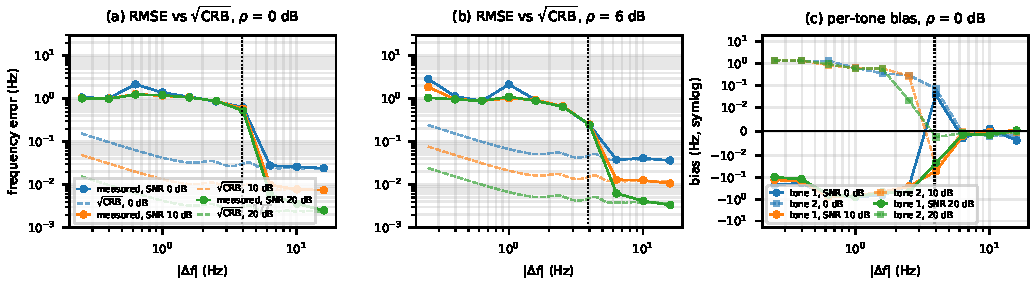
\includegraphics[width=0.68\textwidth]{figures/fig_twotone_crb_wide.pdf}
\caption{Direct validation of Proposition~\ref{prop:crb} ($K{=}2$
carrier-only model): measured spectral-line two-tone estimation vs.\
the exact two-tone CRB. (a),(b)~pooled RMSE (solid) vs.\ $\sqrt{\crb}$
(dashed) at amplitude ratio $0$\,dB / $6$\,dB; (c)~per-tone bias
(symlog, $0$\,dB); vertical line: $1/T_{\mathrm{burst}}$.}
\label{fig:twotone}
\end{figure*}

% ======================================================================
\section{Method: RS-SlotSepNet}
\label{sec:method}

The receiver-structured slot separator (RS-SlotSepNet) keeps the
learned baseline separator of Section~\ref{sec:method-backbone} and
wraps it in the classical receiver stages that
Section~\ref{sec:theory} designates: \emph{separate $\to$ per-slot sync
$\to$ joint re-detection}. E4 assigns each stage its final role
(Section~\ref{sec:e4}).

\subsection{Baseline separator (SlotSepNet)}
\label{sec:method-backbone}

The separator is our own slot-based design, used here as a fixed,
pretrained baseline --- it is not the contribution, and E4 will show it
should not be the detection front-end. A complex-valued convolutional
encoder (complex arithmetic via paired real
operations~\cite{trabelsi2018complex}) feeds four complex residual
blocks with complex squeeze-and-excitation
attention~\cite{hu2018senet}; the representation is read out by
$K_{\max}{=}4$ mask slots, each producing a separated waveform, with a
shared occupancy head scoring slot activity and a count head
aggregating the occupancies ($\approx$254K parameters). Training uses
the benchmark's mixtures ($K \in \{1,2,3\}$; 2000 mixtures/epoch,
batch 16, Adam $10^{-3}$, 100 epochs) with a variable-count
permutation-invariant loss~\cite{kolbaek2017pit} on SI-SDR plus
occupancy cross-entropy and an MSE anchor; five seeds ($42$--$46$)
give the checkpoint population E3/E4 average over. Its quality is
measured, not asserted: on the test grid the separator reaches
SI-SDR improvement $9.6/3.2/2.8$\,dB at $K{=}1/2/3$ with slot
occupancy recall $0.98/0.98/1.00$ (precision $0.89/0.68/1.00$ --- the
$K{=}2$ precision is the surplus-slot behaviour of
Section~\ref{sec:e3}), and two cross-family checks on the same $K{=}2$
cells: the C-SE convolutional separator of our companion work,
evaluated \emph{zero-shot}, reaches SI-SDRi $3.5$\,dB, and the
published CNSE separator~\cite{hou2022single} ($6.7$M parameters,
$26\times$ ours, retrained on the benchmark's $K{=}2$ mixtures, five
seeds) reaches $6.0$\,dB --- so the E3 premise does not hinge on one
architecture, and Section~\ref{sec:e4} prices what the stronger
separator buys the waveform route. The waveform
model's job is only
to hand the receiver per-slot streams whose residual is structured
leakage --- how good those streams are for \emph{detection} is an
empirical question, answered (negatively) by E4's V2 arm.

\subsection{BlindCarrierSync (per slot)}
\label{sec:method-sync}

Each occupied slot's passband burst $\hat{s}(t)$ is synchronised
blindly, with no learning and no oracle input. The residual carrier
offset after down-conversion at the nominal $f_0$ lies in
$[-5, +10]$\,Hz. The final algorithm --- reached by measurement, and
simpler than the textbook pipeline in two places --- is:

\begin{enumerate}
  \item \emph{Coarse down-conversion} at $f_0$.
  \item \emph{Sample-level coarse frequency.} Apply the RRC matched
        filter \emph{first} (a $10.7$\,dB noise-bandwidth reduction that
        is essential: on the raw burst, transition-slew spurs in the
        nonlinearised spectrum exceed the carrier line for 8PSK/16QAM
        even at high SNR), then form the $M$-th power ($M$ the
        rotational symmetry order; phase-only normalisation for PSK,
        amplitude-weighted powers for 16QAM~\cite{viterbi1983nonlinear}).
        The line at $M \Delta f$ is located by an $8\times$ zero-padded
        FFT with parabolic peak interpolation.
  \item \emph{Symbol-level refinement and wrong-peak rescue.} Three
        candidates: the coarse estimate, a narrow ($\pm 2$\,Hz)
        re-estimate around it, and a full-window ($\pm 13$\,Hz)
        re-estimate, all from the $M$-th-power line search on the
        \emph{decimated symbol stream} (256 clean constellation samples
        instead of 4096 slew-corrupted ones). The candidate maximising
        the product of two decision-free coherence scores ---
        sample-level line strength and symbol-level
        $\big|\mathrm{mean}(z^M)\big|$ --- wins; the product works
        because the two scores have disjoint failure modes (deep-fade
        bursts keep a strong sample-level line while symbol-level
        coherence is fooled by ISI, and vice versa).
  \item \emph{Demodulation} with the winning estimate: correction,
        matched filter, symbol grid, unit-power normalisation.
  \item \emph{No decision-directed phase refinement.} The classical DD
        line fit of the decision-referred phase residual is
        \emph{fold-biased} under fading: wrong decisions fold the
        measured phases toward the nearest grid point, biasing the
        fitted intercept ($\approx 6^\circ$) and \emph{increasing} SER
        at high SNR (8PSK at $20$\,dB: $0.028 \to 0.087$). Non-data-aided
        alternatives (Viterbi--Viterbi symbol
        phase, min-distance phase scan) are no better under the 3-tap
        channel. The residual constant phase is small after frequency
        correction and is absorbed by the $M$-fold ambiguity resolution
        of the scoring (differential coding in a deployed system).
\end{enumerate}

Known boundaries, analysed. The $M$-th-power line amplitude at the true
residual factorises as $|\mathbb{E}[c^M]| \cdot |\sum_l h_l^M|$ with
$h_l$ the fading taps (the cross-moments vanish under the alphabets'
rotational symmetry). For PSK, $c^M$ is a deterministic constant ---
$|\mathbb{E}[c^M]| = 1$, zero data self-noise. For 16QAM,
$\mathbb{E}[c^4] = -0.68$: the three amplitude rings contribute
opposite-signed fourth powers, so the coherent line is $3.3$\,dB weaker
and rides on per-symbol self-noise ($\mathrm{Var}(c^4) = 2.66$). Under
the benchmark's 3-tap Rayleigh channel the second factor has mass near
zero ---
$P\big(|\sum_l h_l^4| < 0.15\big) \approx 7\%$ --- and for those bursts
\emph{no} fourth-power method has a usable line (the measured
symbol-level line strength tracks
$|\mathbb{E}[c^4] \sum_l h_l^4|$ with correlation $0.65$).
At
$\snr \leq -5$\,dB the $M{=}8$ line of 8PSK sinks under the noise
floor. Both are intrinsic to short-burst non-data-aided estimation, and
both are reported rather than engineered away (Section~\ref{sec:e1}).

\subsection{JointPairDetector (K = 2)}
\label{sec:method-joint}

Given two synchronised unit-power slot streams $z_{1,n}, z_{2,n}$ and
their modulation hypotheses, the joint log-likelihoods over the
$\leq 16 \times 16$ hypothesis grid are
\begin{equation}
  \ell_n(i, j) = -\big\| z_n - A \, [c_i; c_j] \big\|^2 / \sigma^2,
  \qquad z_n = [z_{1,n}; z_{2,n}],
  \label{eq:jointll}
\end{equation}
with $A \in \mathbb{C}^{2 \times 2}$ the coupling matrix whose columns
absorb the per-source complex gains (Proposition~\ref{prop:discrete}).
$A$ is estimated blind by a classification-EM (hard-EM) procedure from
$A = I$: the E-step makes the joint hard decision \eqref{eq:jointll}
under the current $A$; the M-step is the closed-form complex
least-squares refit $A \leftarrow Z C^{\mathsf{H}}
(C C^{\mathsf{H}})^{-1}$ on the current decisions. Both steps are exact
coordinate optimisations of one least-squares objective, so the
objective is non-increasing per
round (the loop stops at a $10^{-5}$ relative decrease or $30$ rounds).
We call the scheme by its proper
name: classification-EM rather than soft EM with posterior
responsibilities, and --- nested inside the frequency search of
Section~\ref{sec:e4} --- an expectation-conditional-maximisation (ECM)
scheme over the discrete symbols and the continuous
$(A, \Delta f_1, \Delta f_2)$ jointly. Because the landscape at
$\sir \approx 0$\,dB can land in swapped or degenerate
minima, we restart from a small grid over off-diagonal magnitude and
phase (the known operating range $|a_{ij}|/|a_{ii}| \lesssim 1.5$ from
$w_k \sim \mathcal{U}(0.4,0.6)$) and keep the minimum-energy
(maximum-likelihood) solution (same-alphabet pairs retain a near-degeneracy ---
Section~\ref{sec:lim}; E4 measures the effect end to end).

We ran this control: the baseline separator fine-tuned with an
additional differentiable soft-demodulation term (soft constellation
cross-entropy on the PIT-assigned pairs of the baseline loss,
$\lambda_{\mathrm{ser}} \in \{0.1, 1.0\}$, five seeds, the identical
data stream) moves the compensated SER of the E4 waveform route
by at most $0.12$ points ($0.5337 \to 0.5334$/$0.5325$; BER and the
$3.2$\,dB SI-SDR improvement unchanged within seed noise) --- the
tested loss-level modification does not remove the floor of
Theorem~\ref{thm:floor} on this benchmark: within the tested
waveform-separator objective family, the remedy remains structural.
(Architecture-level separator strength is a different lever: E4's CNSE
cross-check, Section~\ref{sec:e4}.)

% ======================================================================
\section{Experiments}
\label{sec:exp}

The benchmark is the variable-$K$ co-frequency test grid of
Section~\ref{sec:model}
(deterministic test seed $99999$; SNR grid $\{-10, \dots, 20\}$\,dB).
The evaluation truth is an offset-compensated receiver ---
true-carrier down-conversion plus phase alignment --- which serves as
the idealised limit any synchroniser is scored against. The operating envelope throughout is
$K \in \{1,2\}$ sources with known modulations --- E5 measures both
boundaries and finds them structural. A note on terminology:
``blind'' here qualifies the \emph{estimate path} --- no oracle
carriers, phases, symbols or modulations are used by any estimator, and
the receiver stages are training-free --- not the operating assumptions,
which are a known nominal carrier and offset range, the benchmark's
fixed timing grid, and per-source modulation knowledge. The receiver is
therefore precisely a \emph{semi-blind, modulation-conditioned}
one. E1--E6 below are complete:
E1--E2 are CPU
and deterministic; E3 ran on the GPU server over the five baseline
separator checkpoints; E4's mixture-route variants (V1/V3/V4) are training-free
and deterministic, and its slot-route variants (V0/V2) share E3's five
checkpoints; E5--E6 are CPU and deterministic.

\subsection{E1: does blind sync approach oracle sync? (complete)}
\label{sec:e1}

On $K{=}1$ test cells (no separation, isolating the synchroniser; $200$
bursts per modulation--SNR cell, two grids) three receivers demodulate
the same bursts against the same reference labels: the \emph{nominal
proxy} (down-conversion at $f_0$, no synchronisation), the
\emph{oracle} compensated receiver, and \emph{BlindCarrierSync} with
the true modulation hypothesis, scored with genie resolution of the
$M$-fold phase ambiguity (Proposition~\ref{prop:discrete}; the
deployment answer, differential coding, is measured in
Section~\ref{sec:lim}).
Table~\ref{tab:e1} reports the per-modulation SER.

\begin{table}[!t]
\centering
\caption{E1: compensated SER per modulation, oracle vs.\ blind carrier
synchronisation ($K{=}1$; $200$ bursts per cell, two test grids; blind
= BlindCarrierSync, genie $M$-fold resolution).
The nominal no-sync proxy sits at $0.62$--$0.69$ at every SNR.}
\label{tab:e1}
\scriptsize
\setlength{\tabcolsep}{3pt}
\begin{tabular}{rcccccccc}
\toprule
& \multicolumn{2}{c}{BPSK} & \multicolumn{2}{c}{QPSK}
& \multicolumn{2}{c}{8PSK} & \multicolumn{2}{c}{16QAM} \\
\cmidrule(lr){2-3}\cmidrule(lr){4-5}\cmidrule(lr){6-7}\cmidrule(lr){8-9}
SNR (dB) & or. & blind & or. & blind & or. & blind & or. & blind \\
\midrule
$-10$ & 0.161 & 0.159 & 0.308 & 0.502 & 0.526 & 0.796 & 0.699 & 0.847 \\
$-5$  & 0.091 & 0.092 & 0.171 & 0.177 & 0.331 & 0.756 & 0.510 & 0.584 \\
$0$   & 0.057 & 0.059 & 0.083 & 0.086 & 0.179 & 0.212 & 0.304 & 0.321 \\
$5$   & 0.029 & 0.030 & 0.049 & 0.053 & 0.101 & 0.124 & 0.164 & 0.189 \\
$10$  & 0.012 & 0.011 & 0.028 & 0.030 & 0.066 & 0.088 & 0.094 & 0.114 \\
$15$  & 0.009 & 0.009 & 0.021 & 0.026 & 0.032 & 0.060 & 0.052 & 0.080 \\
$20$  & 0.007 & 0.007 & 0.009 & 0.012 & 0.018 & 0.054 & 0.027 & 0.065 \\
\bottomrule
\end{tabular}
\end{table}

Blind synchronisation meets its design target --- oracle-level SER ---
for BPSK and QPSK at $\snr \geq -5$\,dB (gaps $\leq 0.5$\,pts; BPSK's
small inversions are reference-label noise). The two honest exceptions
are larger than a low-count pilot suggested: 8PSK runs $2$--$4$ points
above the oracle
at $\snr \geq 0$\,dB --- stable across the two independent grids ---
and 16QAM runs $+2$--$4$ points above it (weak-line bursts and
residual-phase sensitivity; Section~\ref{sec:method-sync}); and the
$M$-th-power line collapses below the noise
floor for 8PSK at $\snr \leq -5$\,dB and for QPSK at $-10$\,dB --- a
physical limit of non-data-aided estimation at $256$-symbol bursts, not
of this particular estimator (where the line survives, the frequency
error is within $1.5\times$ of the CRB;
Fig.~\ref{fig:crb}).

\subsection{E2: theory validation (complete)}
\label{sec:e2}

Fig.~\ref{fig:crb}--\ref{fig:dmin} collect the measurement validation
of Section~\ref{sec:theory}; the Monte-Carlo curves behind
Section~\ref{sec:theory-joint} are in the public code's figure outputs.
The bounds sandwich the
measured operating points: the union bound sits above the joint
Monte-Carlo SER at every phase grid point (asserted computationally),
the exact evaluation \eqref{eq:exactsep} sits on the separate
Monte-Carlo curve (within $0.003$) and converges to the
continuous-ensemble floor \eqref{eq:floor} ($0.4999$ resp.\ $0.8380$),
the marginal-MAP Monte-Carlo removes the joint rule's
low-SNR reversal, and the measured synchroniser errors sit above the CRB
with the expected inefficiency factor. The 16QAM column of the
Monte-Carlo validation is the quantitative reason the end-to-end gain
should be expected on PSK pairs rather than QAM pairs.

\begin{figure*}[!t]
\centering
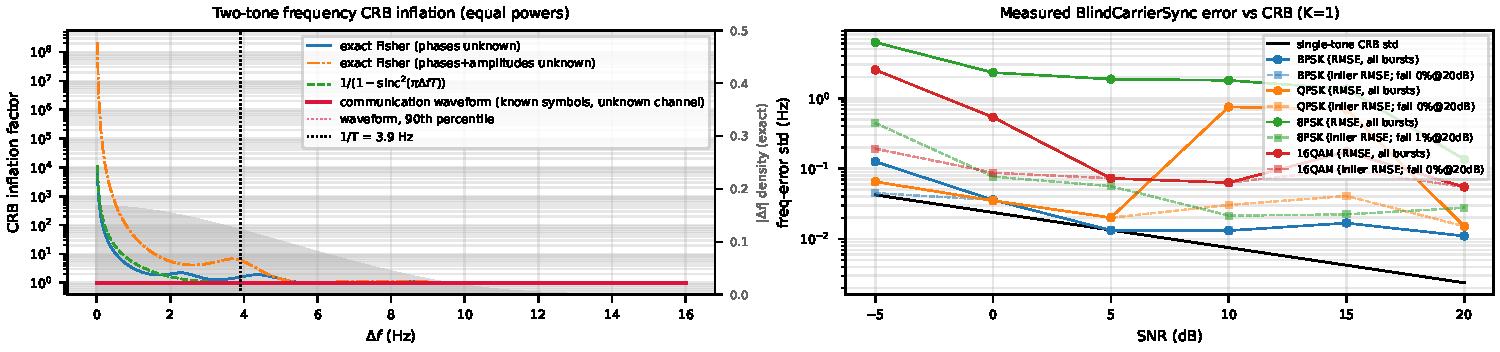
\includegraphics[width=0.57\textwidth]{figures/fig_e2_crb_inflation.pdf}
\caption{Left: exact two-tone frequency-CRB inflation vs.\ offset for
the \emph{carrier-only surrogate}, phases the only nuisance parameters
(solid), resp.\ gains also unknown (dash-dotted); the known-symbol
communication-waveform Fisher matrix
(Remark~\ref{rem:waveform-fim}) shows no coupling (red, near-flat at
$1\times$); sinc$^2$ heuristic (dashed),
$1/T_{\mathrm{burst}}$ (dotted), benchmark $|\Delta f|$ density
(shaded, right axis).
Right: measured BlindCarrierSync error vs.\ single-tone CRB
on $K{=}1$ bursts: all-burst RMSE (solid) and inlier RMSE
(dashed; failures $|\hat{f} - f| > 1$\,Hz excluded, rates in legend).}
\label{fig:crb}
\end{figure*}

\begin{figure}[!t]
\centering
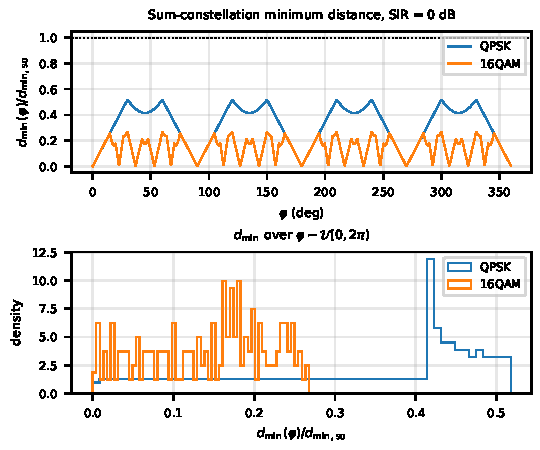
\includegraphics[width=0.85\columnwidth]{figures/fig_e2_dmin_phi.pdf}
\caption{Minimum distance $d_{\min}(\varphi)$ of the sum constellation
at $\sir = 0$\,dB, normalised by the single-user distance (top: the
QPSK curve touches zero at the four commensurate rotations --- at
$\varphi = 90^\circ$, $(c_1, c_2) \mapsto (c_1 + \jj\delta,\, c_2 -
\delta)$ leaves the mixture point invariant for every $\delta$ in the
QPSK difference set; bottom: density over
$\varphi \sim \mathcal{U}[0, 2\pi)$; 16QAM's typical minimum distance
is $6\times$ smaller than QPSK's).}
\label{fig:dmin}
\end{figure}

\subsection{E3: end-to-end blind pipeline (complete)}
\label{sec:e3}

E3 scores the end-to-end pipeline under two receivers sharing one
scoring code. The baseline separator of
Section~\ref{sec:method-backbone} (five seeds, no fine-tuning)
separates each test mixture; the occupied slots (occupancy $> 0.5$,
Hungarian-matched to the true sources on SI-SDR, matched pairs only)
are demodulated by the \emph{oracle} compensated receiver (true-carrier
down-conversion plus phase alignment) or by BlindCarrierSync, scored by
compensated SER/BER with genie $M$-fold rotation resolution
($K \in \{1,2,3\}$, $100$ mixtures per $K \times \snr$ cell, test
seed $99999$).

The oracle arm is already this paper's first empirical result ---
the waveform-to-bit gap, measured directly. With separation in place
and synchronisation idealised away, the pooled SER is $0.5027$
(per-seed range $0.5019$--$0.5037$; BER $0.2651$), but the per-$K$
split shows where that number comes from: $0.1454$ at $K{=}1$ against
$0.5534$/$0.5858$ at $K{=}2$/$3$. At $K \geq 2$ the ideally received
separated streams sit just above the exact separate-detection floor of
Theorem~\ref{thm:floor} ($1/2$ for QPSK pairs at $\sir = 0$\,dB) and
far above the $K{=}1$ level: the separator works as a
waveform model --- its slots match the true sources closely enough to
be Hungarian-paired on SI-SDR --- yet through any separate-then-detect
receiver that quality does not reach the bits. Replacing the oracle
receiver by BlindCarrierSync makes this
strictly worse, and because both arms share the scoring code, every
gap below is attributable to synchronisation alone.

\begin{table}[!t]
\centering
\caption{E3: blind-minus-oracle compensated SER (percentage points,
5-seed mean), per $K$ and SNR. Pooled, the blind arm loses
$+8.5 \pm 0.1$\,pts (population std; $5/5$ seeds positive);
pooled BER degrades $0.2651 \to 0.3519$.}
\label{tab:e3}
\scriptsize
\begin{tabular}{lrrrrrrr}
\toprule
& \multicolumn{7}{c}{$\Delta$SER (pts) at SNR (dB)} \\
\cmidrule(lr){2-8}
$K$ & $-10$ & $-5$ & $0$ & $5$ & $10$ & $15$ & $20$ \\
\midrule
1 & $+14.7$ & $+16.9$ & $+2.3$ & $+2.0$ & $+1.3$ & $+0.7$ & $+1.8$ \\
2 & $+9.7$ & $+10.9$ & $+9.5$ & $+8.1$ & $+8.3$ & $+7.6$ & $+8.1$ \\
3 & $+7.4$ & $+7.9$ & $+9.6$ & $+9.8$ & $+9.7$ & $+10.7$ & $+10.1$ \\
\bottomrule
\end{tabular}
\end{table}

Table~\ref{tab:e3} decomposes the penalty, and the decomposition is the
result. At $K{=}1$ the blind pipeline behaves exactly as E1 predicts:
the gap is $+0.7$--$+2.3$\,pts at $\snr \geq 0$\,dB and blows up only
at $-10$/$-5$\,dB, where the $M$-th-power line sinks below the noise
floor (Section~\ref{sec:e1}). At $K \geq 2$ the gap is instead
\emph{SNR-flat}: $+8$--$+11$\,pts at every SNR from $-10$ to
$20$\,dB. The mechanism is visible in the synchroniser's own error
statistics: the median blind frequency error on $K \geq 2$ slots is
$2$--$4$\,Hz at \emph{every} SNR (against $0.007$--$0.04$\,Hz on
$K{=}1$ slots at $\snr \geq 0$\,dB). The residual interferer leaking
into each slot
carries its own $M$-th-power spectral line, and that line \emph{pulls}
the per-slot carrier estimate off the true carrier --- a structured,
SNR-independent bias, not noise. Two controls pin the mechanism down.
First, a crude successive-interference-cancellation variant (sync each
slot after subtracting the other matched slots from the mixture) does
not help: pooled $K{=}2$ SER $0.6484$ vs.\ $0.6422$ for plain blind
sync --- the subtracted estimates are themselves biased. Second, and
decisively, blindly synchronising the \emph{raw mixture} at $K{=}2$
scores $0.6427$, statistically indistinguishable from the
separate-then-sync pipeline's $0.6422$: separation followed by
\emph{independent} synchronisation buys nothing over no separation.
This is precisely the phase/frequency-entanglement regime of
Propositions~\ref{prop:gauge}--\ref{prop:discrete}: per-slot the
interferer-rotated constellation is itself a valid hypothesis, so the
carrier estimates cannot be disentangled slot by slot. E3 is thus the
motivational negative for E4 --- synchronisation and detection must be
joint, and must face the interference, not a separated proxy of it.

\emph{End-to-end accounting.} The per-pair SERs above are conditional
on successful source--slot matching; a receiver's deliverable is bits,
so misses and phantom slots must be priced. Re-running with per-sample
accounting (five checkpoints, same grid) gives:
source-count accuracy $0.909/0.042/1.000$ at $K{=}1/2/3$ (pooled
$0.650$) --- the occupancy head lights a surplus third slot on $93\%$
of $K{=}2$ mixtures --- but the counting errors are almost entirely
\emph{false-alarm slots} that Hungarian matching
discards (per-source miss probability $2.3\%/1.5\%/0\%$). The separator's measured value is
therefore \emph{localisation and slot generation}, not
\emph{counting}: the learned count head
is unreliable at $K{=}2$ ($4.2\%$), and any counting use must
threshold the occupancy head. Pricing a missed source as a total
detection failure (SER $1$, BER $0.5$ for that source), the
end-to-end SER moves the oracle arm to $0.165/0.560/0.586$ per $K$
(from $0.145/0.553/0.586$ conditional) and the blind arm to
$0.218/0.648/0.679$ (from $0.200/0.642/0.679$) --- both gaps widen by
$\leq 0.7$ points at $K{=}2$ --- none of the conclusions above is an
artefact of the matched-pairs conditioning.

\subsection{E4: joint sync and detection at \texorpdfstring{$K{=}2$}{K=2} (complete)}
\label{sec:e4}

E4 tests whether closing the loop --- estimating both carriers, both
complex gains and the symbol pair \emph{jointly} --- converts the
headroom of Theorem~\ref{thm:ub} into bits. Five variants share the
same scoring (per-source SER, PIT- and $M$-fold-rotation-resolved;
$K{=}2$ test cells, $100$ mixtures per SNR; V0/V2 on the reference
grid, test seed $99999$, cross-checked by an independent server run;
the deterministic variants V1/V3/V4 run on five independent test
grids, seeds $99999$/$88888$/$77777$/$55555$/$31337$, so the headline
contrasts carry seed-level confidence intervals):

\begin{itemize}
  \item \textbf{V0, naive chain.} E3's blind-synced slot streams fed to
        the EM-$A$ JointPairDetector (Section~\ref{sec:method-joint};
        five baseline checkpoints).
  \item \textbf{V1, ECM on the raw mixture.} Joint sync and detection
        directly on the unseparated mixture: an ECM loop alternates
        joint symbol decisions on the $\leq 16 \times 16$ grid
        \eqref{eq:jmap} with complex least-squares gain/phase refits,
        nested in a coarse-to-fine frequency search with converged
        classification-EM at every candidate and an NLS polish ---
        Appendix~\ref{app:alg} gives the full procedure,
        its monotonicity
        argument and its convergence criteria. Training-free; no
        separator involved; $\approx 1.6$\,s per burst together with
        V4 on one CPU core (measured).
  \item \textbf{V2, slot-aided ECM.} The same ECM loop fed with the two
        occupancy-top slot streams as a two-channel observation (five
        checkpoints) --- the architecture of Section~\ref{sec:method}.
  \item \textbf{V3, oracle-frequency reference.} V1 with the frequency
        search replaced by the true carrier offsets; a reference arm
        quantifying the residual acquisition cost (not a bound: gains
        and symbols are still estimated under the finite-tap model).
  \item \textbf{V4, ISI-aware ECM.} V1 warm-started, with the
        memoryless observation model replaced by a per-source
        $L{=}5$-tap \emph{centred} symbol-rate response
        $r_n = \sum_k \ee^{\jj 2\pi \Delta f_k n T_s}
        \sum_{l=0}^{L-1} g_k[l]\, c_{k,\, n-(l-\lfloor L/2 \rfloor)}$
        (centred matches the generator's zero-delay fading; $L{=}7$
        saturates): parallel-iterated ISI cancellation with joint grid
        decisions, a closed-form $2L$-tap least-squares refit, and a
        tap-aware NLS frequency polish; energy-monotone by an explicit
        accept/fallback test against V1 (never triggered).
        $\approx 1.6$\,s per burst together
        with V1 on one CPU core. V1 is exactly V4 with $L{=}1$, so the
        V4--V1 contrast doubles as the memoryless-model ablation.
\end{itemize}

\begin{table*}[!t]
\centering
\caption{E4: per-source SER on the $K{=}2$ test cells. V0/V2 average
over the five separator checkpoints on the reference grid (test seed
$99999$); V1/V3/V4 are deterministic per grid and average over
\emph{five independent test grids} (seeds
$99999$/$88888$/$77777$/$55555$/$31337$; $95\%$ seed-level CIs
$\pm 0.004$/$0.004$/$0.005$ for V1/V4/V3); marginal-MAP re-decision
changes nothing (V1 $0.5388$ vs.\ $0.5392$; V3 $0.4101$ vs.\ $0.4106$).
The reference rows are the waveform route (separate, oracle sync),
symbol-wise and with per-slot PSP/Viterbi ($5$-checkpoint means), and
the same PSP route with the separator replaced by the retrained
published CNSE~\cite{hou2022single};
blind demodulation of the raw mixture scores $0.6427$. The last column
is the pooled Gray-mapped BER (same decisions).}
\label{tab:e4}
\setlength{\tabcolsep}{3pt}
\scriptsize
\begin{tabular}{lrrrrrrrrr}
\toprule
& \multicolumn{7}{c}{SER at SNR (dB)} & & \\
\cmidrule(lr){2-8}
Variant & $-10$ & $-5$ & $0$ & $5$ & $10$ & $15$ & $20$ & pooled &
BER \\
\midrule
V0 slots $\to$ blind sync $\to$ EM-$A$ &
  0.674 & 0.628 & 0.634 & 0.559 & 0.590 & 0.590 & 0.580 & 0.6078 &
  0.353 \\
V1 ECM on raw mixture &
  0.688 & 0.628 & 0.554 & 0.518 & 0.474 & 0.458 & 0.455 & $0.5392$ &
  $0.312$ \\
V2 ECM on slot streams &
  0.702 & 0.660 & 0.634 & 0.547 & 0.531 & 0.550 & 0.548 & 0.5960 &
  0.354 \\
V4 ISI-aware ECM ($L{=}5$) &
  0.689 & 0.628 & 0.551 & 0.510 & 0.461 & 0.441 & 0.438 & $0.5310$ &
  $0.306$ \\
V3 oracle-frequency ECM &
  0.608 & 0.522 & 0.422 & 0.374 & 0.331 & 0.315 & 0.303 & $0.4106$ &
  $0.215$ \\
\midrule
waveform route, oracle sync, symbol-wise &
  0.592 & 0.555 & 0.564 & 0.526 & 0.544 & 0.548 & 0.540 & 0.5527 &
  0.285 \\
waveform route, oracle sync, PSP/Viterbi &
  0.585 & 0.537 & 0.545 & 0.493 & 0.526 & 0.527 & 0.522 & 0.5337 &
  0.266 \\
waveform route, CNSE separator, oracle sync, PSP &
  0.580 & 0.508 & 0.488 & 0.372 & 0.410 & 0.378 & 0.373 & 0.4440 &
  0.213 \\
\bottomrule
\end{tabular}
\end{table*}

\emph{Statistical reporting.} The unit of inference throughout E4 is
the mixture burst: each of the five independent test grids holds
$7$ SNR values $\times$ $100$ bursts $= 700$ bursts, and pooled SERs
aggregate all bursts of a route ($95\%$ CIs over the five grids).
Paired contrasts use the paired per-burst difference of two routes on
the same bursts: the V1--V4 contrast pools all $3500$ paired bursts of
the five grids, while the headline waveform-route contrast pairs the
$700$ bursts of the reference grid (seed $99999$), the route arm
averaged over its five separator checkpoints per burst. For every
paired contrast we report a paired-bootstrap $95\%$ CI of the
\emph{mean} per-burst difference together with a Wilcoxon signed-rank
$p$-value; the two target different estimands --- the mean gap versus
symmetry of the paired differences about zero --- so a bootstrap
interval containing zero can coexist with a significant Wilcoxon $p$,
as for the headline contrast below. A tie is claimed only when the
paired interval contains zero.

\emph{Results.} Table~\ref{tab:e4} orders the variants as sanity
demands, V3 $<$ V4 $<$ V1 $<$ V2 $<$ V0, and delivers three findings.
First, the headline, which the paired tests make precise. The
training-free joint loop on the raw mixture \emph{ties the strongest
waveform route at the paper's separator quality}: pooled SER $0.5310$ (V4, $95\%$ CI
$[0.5261, 0.5360]$ over five independent test grids) against $0.5337$
for the oracle-received waveform route upgraded with per-slot
PSP/Viterbi sequence detection (decision-directed $L{=}3$ channel
estimation; $0.5527$ for its symbol-wise special case) --- the
route-minus-V4 paired per-burst difference is $+0.003$ with $95\%$ CI
$[-0.011, +0.018]$
(Wilcoxon $p{=}4.8\times 10^{-4}$; $n{=}700$ paired bursts) --- while
using no oracle carriers, phases or symbols during inference,
against $0.6427$ for blind
demodulation of the unseparated mixture ($-11.2$\,pts). The contrast
is SNR-structured, and the structure is the content: at
$\snr \leq 0$\,dB the oracle-assisted separate routes win by
$4$--$11$ points (their advantage is the oracle synchroniser, not the
architecture), while at $\snr \geq 5$\,dB the blind joint loop wins
by $+0.03$--$+0.10$; the memoryless special case V1 already ties the
PSP route ($0.5392$, CI $[0.5342, 0.5441]$). The bit-level view
(pooled Gray-mapped BER, Table~\ref{tab:e4}) is more nuanced: V4's
$0.306$ trails the PSP route's $0.266$ pooled --- the 16QAM-involving
pairs carry four bits per symbol and no route recovers them --- while
on PSK-only pairs V4 leads ($0.236$ vs.\ $0.250$), mirroring the SER
structure. Removing the scoring genie entirely ---
differential-equivalent decoding on the PSK-pair bursts ($n{=}383$,
same decisions pipeline) --- turns the tie into a clear win: V4 holds
at $0.372$ SER / $0.244$ BER while the PSP route degrades to
$0.537$ / $0.357$: differential detection tolerates the joint loop's
residual acquisition error but punishes the waveform route's error
structure. The architecture
contrast, isolated from acquisition by the oracle-frequency arm, is
larger: V3 beats the oracle-received PSP route by $12$ pooled points
($0.4106$ vs.\ $0.5337$), growing to $+22$ points at $20$\,dB ---
joint detection, not synchronisation, is where the headroom lives.

\emph{Cross-architecture check (CNSE).} Is the waveform route's
ceiling set by our separator rather than the architecture? We
retrained the published CNSE separator~\cite{hou2022single} ($6.7$M
parameters, $26\times$ ours, $K{=}2$-specialised training; SI-SDRi
$6.0$\,dB vs.\ $3.2$\,dB) and ran
it through the identical route (Table~\ref{tab:e4}, last row). The
route improves by $9$ pooled points ($0.5337 \to 0.4440$; BER $0.266
\to 0.213$): it is separator-quality-limited, and
Theorem~\ref{thm:floor}'s floor is confirmed as a property of the
linear-residual regime it models, not of separation as such ---
consistent with the true-stream control ($0.041$).
(i)~At \emph{matched}
oracle frequencies the joint loop still wins: V3 $0.4106$ vs.\
$0.4440$. (ii)~The CNSE route's advantage is entirely the oracle
synchroniser: replacing it by per-slot blind sync costs $+9.2$ pooled
points ($0.5356$) --- inside E3's $+8$--$11$ capture band, with the
interferer's line still capturing $36$--$45\%$ of bursts at
$\snr \geq 5$\,dB despite the $6$\,dB cleaner slots --- so
blind-versus-blind the joint loop again ties the strongest waveform
route ($0.5310$ vs.\ $0.5356$). (iii)~Under genie-free differential
scoring (PSK pairs) the joint loop leads \emph{every} waveform route:
V4 $0.372$ vs.\ CNSE oracle-PSP $0.438$ and CNSE blind-PSP $0.442$.
Second, V0 is
worse than the waveform route it augments ($0.6078$ vs.\ $0.5534$):
chaining the biased
per-slot sync of E3 into the joint detector poisons it, confirming
that the E3 failure is in the sync stage, not the detector. Third, V2
--- the slot-aided architecture --- loses to V1 by $+5.8$\,pts,
positive on all $5/5$ seeds ($+4.3$\,pts against the waveform-route
reference, also $5/5$). Direct measurement on $40$ held-out $K{=}2$
bursts at $20$\,dB explains why: the
mask-separated slot streams carry $1.6$--$1.84\times$ the mixture's
converged-ECM residual energy per channel-symbol (PSK pairs: median
$0.0274$ vs.\ $0.0122$; 16QAM-involving: $0.0297$ vs.\ $0.0148$) ---
mask separation distorts the linear two-source superposition that the
ECM likelihood assumes, and the distortion costs more than the leakage
suppression buys (within-burst gain drift is also $\approx 1.5\times$
larger on the slots). The positive control is the same ECM loop on the
two \emph{true} source streams: SER $0.041$ vs.\ $0.121$ for
mixture-ECM on the same bursts --- the joint loop would win decisively
if the separation were clean. At the current separator quality
it is not, and the operating answer on this benchmark is: joint
detection should run on the mixture; separation serves slot generation
and localisation, not detection (its learned count head is unreliable
at $K{=}2$; Section~\ref{sec:e3}). The remaining V4--V3 gap ($0.531$ vs.\
$0.411$) is the frequency-acquisition residual, the price of
Proposition~\ref{prop:crb}'s two-tone inflation paid once, jointly,
instead of twice, per slot.

\emph{Where the gain lives.} Splitting the pool by
alphabet pair: on PSK-only pairs V4 reaches $0.378$ (V1: $0.390$; V3:
$0.254$), while 16QAM-involving pairs sit at $0.726$, essentially
unchanged from V1's $0.729$ (V3: $0.610$) --- exactly the
concentration E2's
$d_{\min}(\varphi)$ analysis predicted (Section~\ref{sec:e2}): for
16QAM-involving pairs the dense sum constellation leaves no headroom at
the burst SNRs, and neither joint detection nor ISI modelling can
change that. The pooled figure therefore understates the joint
loop's gain on constant-modulus constellations.

\emph{The SNR curve is non-monotone} (V1 best at $10$\,dB, rising again
toward $20$\,dB): below the knee the loop is noise-limited; above it,
the memoryless two-source model~\eqref{eq:symrate} itself is the
floor. V4 confirms the attribution with a
signature rather than a single number: the share of the V1$\to$V3 gap
that V4 closes on PSK-only pairs grows monotonically from $1\%$ at
$-10$\,dB to $20\%$ at
$20$\,dB ($3/7/15/14\%$ in between) --- an ISI floor must vanish when
noise dominates and dominate when noise vanishes, and it does; the
$20$\,dB PSK floor itself moves $0.2408 \to 0.2169$. A reference
check with oracle frequencies on $20$\,dB QPSK pairs isolates the same
budget: the $L{=}5$ loop reaches $0.106$ vs.\ $0.164$ for the
memoryless oracle (true-stream control: $0.041$). V4's pooled margin over V1
($0.5310$ vs.\ $0.5392$) is small precisely because the budget it
attacks only opens at high SNR and on PSK pairs --- but it is
statistically solid (paired per-burst CI $[+0.0074, +0.0089]$,
$p \approx 10^{-90}$, $n{=}3500$ paired bursts) and it costs
nothing elsewhere (energy-monotone, zero fallbacks,
Table~\ref{tab:e4}).

\emph{Implementation remarks.} The EM inside the frequency search must run
\emph{to convergence} at every ranked candidate (truncated, the
residual-energy ranking is inverted); every frequency move must be
re-evaluated with EM re-converged (a decision-frozen NLS cannot leave
a bad-decision basin); the gain-phase initialisation must cover one
symmetry sector finely. Measured and rejected:
$M$-th-power extreme-lines frequency estimation (cross terms /
interferer power dominate at
$\sir \approx 0$\,dB) and decision-directed frequency refinement
(decision flips create false spectral lines).

\subsection{E5: blind modulation, $K{=}3$ probe, and ablations (complete)}
\label{sec:e5}

E5 measures the two boundaries of the operating envelope --- blind
modulation handling and $K \geq 3$ --- and ablates the joint loop's
moving parts. Both boundary measurements are negative, and both are
measured, not assumed.

\emph{Blind modulation-pair selection (V4B).} Everything reported so
far conditions on the true modulation pair. Lifting that assumption
means choosing among the $10$ unordered pairs, each arm costing a full
ECM fit. Three selectors --- the raw converged energy, the
held-out (even/odd) energy, and the unnormalised soft evidence ---
collapse onto the densest hypothesis, picking
(16QAM, 16QAM) on essentially every burst: the overfit lives in the
per-symbol minimum over a dense grid and no held-out scoring fixes it.
Per-hypothesis-$\sigma^2$ evidence overcorrects into
always-(BPSK, BPSK), and the per-source lock-score two-stage inherits
E1's density bias. The one
working selector is \emph{normalised} soft evidence: log-sum-exp over
the hypothesis grid minus the term-count penalty $\log(M_1 M_2)$, with
a shared $\sigma^2$ from the best fit. Even with it, the joint
classify-and-detect pipeline (wrong pair $\Rightarrow$ SER $1$) reaches
pair accuracy of only $0.11/0.53/0.40$ at SNR $0/10/20$\,dB
(chance $0.10$) and end-to-end SER $0.987/0.610/0.762$, pooled $0.786$
against $0.483$ for known-modulation V4 on the same cells.
The per-pair breakdown is the diagnostic: at $10$\,dB the
PSK-only pairs are identified reliably ($0.86$--$0.88$) while
16QAM-involving pairs sit at $0.11$--$0.78$; at $20$\,dB the selector drifts
toward 16QAM-involving hypotheses --- the density bias of the evidence
measure reasserting itself where the noise no longer masks it.
Conditional on a correct pair decision the detector is intact
($0.880/0.264/0.404$ by SNR). The tested evidence-based selectors are
insufficient: what is missing is a receiver \emph{stage} (a dedicated
modulation-recognition front-end), so known modulation remains the
operating assumption (Section~\ref{sec:lim}).

\emph{$K{=}3$ feasibility probe.} Extending the joint loop to three
sources (sequential-extraction initialisation: a $K{=}2$ ECM fit,
subtraction, an $M$-th-power line search for the third carrier; then a
three-source converged phase-grid EM with centred $L{=}3$ taps and PIT
over the six assignments) fails \emph{at the acquisition stage we
tested}: on PSK-only triplets ($13$ and $8$ cells at SNR $5$ and
$15$\,dB) the resulting $K{=}3$ ECM scores $0.622/0.572$ against the
same-cells oracle mixture baseline's $0.516/0.458$ --- the $K{=}2$ fit
locks a phantom pair, after which the residual's $M$-th-power line is
meaningless. We
state the negative precisely: the \emph{tested} $K{=}3$ acquisition
strategy --- sequential extraction plus $M$-th-power line search --- is
unreliable; whether a different acquisition stage (e.g.\ a joint
three-tone grid) makes $K{=}3$ feasible is open, and no impossibility
is claimed. This paper's scope is
$K \in \{1,2\}$ --- $K{=}1$ by BlindCarrierSync, $K{=}2$ by V4.

\emph{Ablations.} On a subset of the $K{=}2$ grid (SNR
$\{0, 10, 20\}$\,dB, $25$ cells per SNR, test seed $99999$;
deterministic) the NLS polish contributes nothing
($+0.2$\,pp), dropping the restart set to the top-$1$ coarse candidate
costs $0.8$\,pp, and the ISI taps show the expected dose-response,
SER falling monotonically from $L{=}1$ (V1, $0.5202$) through
$L{=}3$ ($0.5130$) to $L{=}5$ ($0.5077$) --- the V4 gain
is carried by the channel model, not any single implementation choice.

\subsection{E6: robustness sweeps (complete)}
\label{sec:e6}

Three sweeps probe the boundaries of the operating assumptions
($K{=}2$, QPSK$+$QPSK, $100$ bursts per cell, deterministic;
Fig.~\ref{fig:robust}). \emph{Carrier separation}
($|\Delta f| \in \{0, \dots, 8\}$\,Hz): the end-to-end SER is
remarkably flat in $|\Delta f|$ --- the joint likelihood search
substitutes for spectral-line acquisition, exactly the route
Remark~\ref{rem:waveform-fim} says the modulation structure enables
--- while the frequency RMSE stays elevated at co-frequency and the
V4--V3 acquisition gap is largest at $\Delta f = 0$ ($0.047$ at
$20$\,dB), vanishing by $8$\,Hz, where the ISI-aware model beats the
memoryless oracle by $3.5$ points. \emph{Timing offset}
($\tau \in \{0, 0.1, 0.25, 0.5\}\,T_s$): graceful to $0.1\,T_s$
($+0.005$--$+0.04$ SER), collapsing at $0.25\,T_s$ ($0.58$ at high
SNR) and near-random at $0.5\,T_s$ --- the symbol-rate model assumes
the zero-delay grid, so timing recovery is a required deployment
stage, and its sensitivity is now measured rather than assumed.
\emph{Amplitude ratio} ($\rho \in \{-10, \dots, 10\}$\,dB): graceful
within $\pm 5$\,dB, weak-source-limited at $\pm 10$\,dB
($0.43$--$0.48$ at high SNR) --- this is also the end-to-end SIR
sweep: joint detection is best at $\sir \approx 0$\,dB, the
benchmark's operating point, and the weak stream becomes
undecodable as $|\rho|$ grows.
\begin{figure*}[!t]
\centering
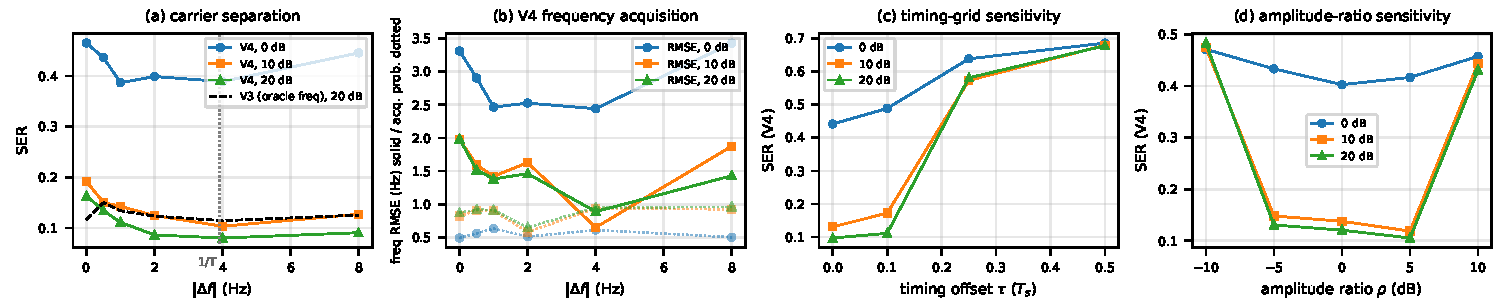
\includegraphics[width=0.57\textwidth]{figures/fig_e6_robustness.pdf}
\caption{Robustness sweeps of the V4 joint loop ($K{=}2$, QPSK$+$QPSK,
$100$ bursts per cell; V3 is the oracle-frequency reference).
(a)~SER vs.\ carrier separation $|\Delta f|$.
(b)~V4 frequency RMSE (solid) and acquisition probability (dotted)
vs.\ $|\Delta f|$. (c)~SER vs.\ timing-grid offset $\tau$. (d)~SER vs.\
amplitude ratio $\rho = 20\log_{10}(w_2/w_1)$.}
\label{fig:robust}
\end{figure*}

% ======================================================================
\section{Discussion}
\label{sec:disc}

\emph{Three layers, three statistical objects.} The results organise
into one statement: waveform-fidelity optimisation, independent
synchronisation, and per-source detection optimise different
statistical objects. Layer 1 (waveform vs.\ bits): SI-SDR
does not control SER --- E3 measures the gap directly. Layer 2
(synchronisation): at co-frequency, independent per-source frequency
estimation is information-poor (Proposition~\ref{prop:crb}) and the
effective coefficients are identifiable only jointly
(Proposition~\ref{prop:discrete}). Layer 3 (detection geometry): the
joint detector's SER is governed by $d_{\min}(\varphi)$ of the sum
constellation while separate detection has an exact, computable floor
(Theorems~\ref{thm:ub}--\ref{thm:floor}). Each layer is closed by a
different structure: the third by joint detection on the mixture, the
second by the same loop's decision feedback, the first
by nothing that waveform-level training alone provides.

\emph{From theory to bits.} E3 measures the
waveform-to-bit gap directly: a working learned separator, read through
an idealised oracle receiver, still sits near the separate-detection
floor at $K \geq 2$ --- the gap is interference-structural, not a
matter of synchronisation quality --- and the theory makes the
structure exactly computable: the floor
(Theorem~\ref{thm:floor}) is the analytic form of the measured flatness,
and the union bound (Theorem~\ref{thm:ub}) with the measured
$d_{\min}(\varphi)$ landscape is the analytic form of the headroom. E3
and E4 then converted the theory into an operating design. The
separate-then-sync chain fails at $K \geq 2$ for exactly the reason
Proposition~\ref{prop:discrete} names --- per slot, the
interferer-rotated constellation is a valid hypothesis, so the
interferer's spectral line captures the slot's carrier estimate
($2$--$4$\,Hz median bias, SNR-flat) --- and the fix is not a better
per-slot synchroniser but the joint loop the identifiability analysis
points to. That loop, run on the raw mixture, ties the strongest
waveform route at the paper's separator quality with no oracle information
during inference, and --- the cleanest architecture contrast --- beats
it by $12$ pooled points when both are given oracle frequencies
($0.411$ vs.\ $0.534$), the gain concentrated on PSK pairs as the
$d_{\min}(\varphi)$ landscape predicts. A retrained published CNSE
separator~\cite{hou2022single} ($26\times$ the parameters, SI-SDRi
$6.0$ vs.\ $3.2$\,dB) does not overturn the contrast: its route
reaches $0.444$ only through the oracle synchroniser (blind:
$0.536$) and trails the joint loop at matched oracle frequencies
($0.411$) and under genie-free scoring ($0.438$ vs.\ $0.372$;
Section~\ref{sec:e4}).
The slot-aided variant's defeat is equally informative: it prices
mask-separation distortion against leakage suppression, and the
true-stream control (SER $0.041$) says the price flips sign once
separation improves --- a concrete target for the next separator.

\emph{Two error budgets, separately quantified.} The
V1$\to$V4$\to$V3 ladder ablates the receiver's
own model (V1 $=$ V4 with $L{=}1$; V3 $=$ V1 with oracle carriers), so
its rungs decompose the distance from the headline number to the
oracle-frequency reference:
the \emph{model budget} (fading ISI the memoryless
likelihood does not span) is worth $0.8$ pooled SER points, growing to
$20\%$ of the PSK-pair gap at $20$\,dB; the \emph{acquisition budget}
(blind two-tone frequency estimation under
Proposition~\ref{prop:crb}'s inflation) dominates at $12$ pooled points
and is where any further headroom lives.

% ======================================================================
\section{Limitations}
\label{sec:lim}

(i) Scoring resolves the residual $M$-fold phase ambiguity by a genie;
the deployment answer is differential coding, measured rather than
assumed (E1-D, $K{=}1$: it removes the genie and is even \emph{more}
robust than genie-resolved decoding at low SNR --- 8PSK at $-5$\,dB,
$0.458$ vs.\ $0.747$ --- and at $20$\,dB it costs $+0.03$--$+0.08$ SER
points, a penalty the oracle receiver pays equally, so the cost is
intrinsic to differential detection, not to synchronisation; at
$K{=}2$ the same pricing is route-dependent --- V4 is flat on PSK
pairs ($0.381 \to 0.372$) while the oracle-assisted waveform route pays
$+9.8$ points ($0.440 \to 0.537$), Section~\ref{sec:e4}).
The synchroniser fails
wholesale for 8PSK below $-5$\,dB SNR; its 16QAM gap of $+2$--$4$ SER
points at high SNR is dominated by weak-line bursts and residual-phase
sensitivity. (ii) Known modulation is an operating
assumption of the whole pipeline, not just of E1: E5's blind
modulation-\emph{pair}
classification at $K{=}2$ reaches $0.11$--$0.53$ accuracy (chance
$0.10$; $100$ cells per SNR) under every selector tried, costing
end-to-end SER $0.786$ vs.\
$0.483$ known-modulation; conditional on a correct pair the detector
itself is intact, so the missing component is a
modulation-recognition stage, which this paper does not build.
(iii) EM estimation of the coupling matrix is only partially
effective for same-alphabet pairs. (iv) The timing grid is fixed by
benchmark construction; a deployment version needs timing
recovery --- the measured sensitivity (Section~\ref{sec:e6}) is
graceful to $0.1\,T_s$ and collapses by $0.25\,T_s$. (v) The E4 loop models fading ISI only as $L{=}5$
symbol-rate taps at the fixed zero-delay grid: the SNR curve remains
mildly non-monotone (V4 best at $10$\,dB), the long-tail residual the
taps do not span is visible in the oracle-frequency check ($0.106$ vs.\
the true-stream $0.041$), and 16QAM-involving pairs admit no gain at
any SNR. (vi) The ECM loop costs $\approx 1.6$\,s per burst per V1$+$V4
evaluation on one CPU core
(a 12th-generation Intel i5;
the per-candidate cost is linear in $N$ and
$M_1 M_2$ and the
joint hypothesis set grows as $\prod_k M_k$ --- exponential in $K$,
the concrete scaling reason $K{=}3$ must change acquisition structure,
Section~\ref{sec:e5}). The loop is an
offline proof-of-concept receiver, not a real-time one: $1.6$\,s per burst is
$\approx 6\times$ the burst duration ($0.256$\,s), the measured peak
resident set is $\approx 0.2$\,GB, and the loop is
numpy CPU code, so a GPU accelerates only the separator forward pass,
not the joint loop. (vii) V1/V3/V4 are deterministic and
training-free,
so their evaluation randomness is the test grid itself; we quantify
it by re-running E4 on five independent test grids (the seed spread is
in Table~\ref{tab:e4}), while the V0/V2 variance comes from the
separator checkpoints only.
(viii)~$K \geq 3$ is out of scope: the
sequential frequency acquisition locks a phantom pair on three-source
mixtures, and the $K{=}3$ probe trails the mixture baseline by
$10$--$11$ SER points (Section~\ref{sec:e5}); a genuinely different
acquisition stage is needed. (ix) E3's per-pair SERs are conditional on
successful source--slot matching; Section~\ref{sec:e3} also reports the
unconditional accounting, which changes none of the
qualitative conclusions.

% ======================================================================
\section{Conclusion}
\label{sec:concl}

SC-BSS of co-frequency signals is trained and ranked by waveform
metrics, but the deliverable is bits. On a controlled variable-count
benchmark --- short bursts, comparable powers, known modulations, a
fixed timing grid --- we showed that a working learned separator's
outputs, even under an oracle receiver, sit near the exact
separate-detection floor at $K \geq 2$, and we derived the receiver
structure that closes
the gap: a joint-MAP union bound and exact separate-detection floor
sandwiching the simulated operating points, a finite-symmetry
identifiability result making synchronisation and joint detection
inseparable in
the co-frequency regime, and an exact two-tone CRB inflation with its
communication-waveform Fisher counterpart locating
the disambiguating information in the modulation-bearing waveform
(reachable by symbol-aware processing). The blind
carrier
synchroniser matches an oracle receiver within $0.5$ SER points at
$\snr \geq -5$\,dB for BPSK/QPSK bursts ($2$--$4$ points for 8PSK),
removing the oracle assumption from the
evaluation pipeline at $K{=}1$ --- and the end-to-end experiments
show why that is not enough: at $K \geq 2$ independent per-slot sync is
captured by the interferer's spectral line (SNR-flat $+8$--$11$ SER
points, no better than no separation --- reproduced with a $26\times$
larger published separator), while a training-free,
ISI-aware ECM joint synchroniser-detector on the raw mixture ties
the strongest waveform route at the separator quality we can reach
(separate, oracle-synced,
PSP/Viterbi sequence detection; $0.531$ vs.\ $0.534$) with no oracle
information during inference, beats the symbol-wise oracle route at
high SNR, and leaves blind mixture demodulation $11$ points behind
($0.643$); the CNSE-built route reaches $0.444$ only through
its oracle synchroniser (blind: $0.536$) and trails the
oracle-frequency joint reference ($0.411$). On this benchmark and at
the separator quality we can currently reach, separation serves
slot generation and localisation, while detection belongs on the mixture,
jointly with synchronisation --- a boundary, not a law: the
true-stream control (SER $0.041$) shows the joint loop would win
decisively again once a separator preserves the linear mixture model
faithfully enough. From the other side, blind modulation-pair
classification fails at the classifier while the detector underneath it
is intact, and the tested $K{=}3$ acquisition strategy fails by
phantom-pair lock
--- two capabilities the tested selector and acquisition strategies
do not provide. The operating envelope is
$K \in \{1,2\}$ with known modulations, and every quantitative claim
is made under the considered short-burst, comparable-power,
known-modulation, fixed-timing co-frequency regime. The remaining gaps
are each quantified and point to concrete next steps (richer channel
structure in the joint loop, and separators trained for mixture-model
fidelity rather than waveform metrics).

% ======================================================================
\appendices
\scriptsize
\section{Proofs of Theorems~\ref{thm:ub}--\ref{thm:floor} and
Propositions~\ref{prop:gauge}--\ref{prop:crb}}
\label{app:proofs}

\begin{proof}[Proof of Theorem~\ref{thm:ub}]
Conditioned on the transmitted pair $c = (c_1, c_2)$, the pairwise
error event $\{c \to c'\}$ is a binary Gaussian test at distance
$D = |\Delta c_1 + a_2 \ee^{\jj\varphi} \Delta c_2|$ in
$\mathcal{CN}(0, \sigma^2)$ noise, hence has probability
$\VQ(D/\sqrt{2\sigma^2})$. The event $\hat{c}_1 \neq c_1$ is the union
of pairwise events with $c_1' \neq c_1$; the union bound and averaging
over the $M_1 M_2$ equiprobable hypotheses give \eqref{eq:ub}.
\end{proof}

\begin{proof}[Proof of Theorem~\ref{thm:floor}]
Condition on $(c_2, \varphi)$: the per-axis received value is
$\ell_i + u + \nu$, $\nu \sim \mathcal{N}(0, \sigma_r^2)$, and level
$i$ is decided wrongly when it crosses the nearest boundary --- above
$b_i$ with probability $\VQ((b_i - \ell_i - u)/\sigma_r)$ ($i < L$),
below $b_{i-1}$ with probability $\VQ((\ell_i + u - b_{i-1})/\sigma_r)$
($i > 1$). Averaging the two events over the $L$ equiprobable levels
gives \eqref{eq:exactsep}; the axes are conditionally independent, so
$P_{e,\mathrm{sep}} = \mathbb{E}[1 - (1-e(u_I))(1-e(u_Q))]$. For the
QPSK floor at $\sir = 0$\,dB: $\ell = \pm 1/\sqrt{2}$, boundary $0$,
$|a_2| = 1$, and with $\theta = \varphi + \arg c_2$ the offsets are
$u_I = \cos\theta$, $u_Q = \sin\theta$ (signs immaterial). As
$\sigma^2 \to 0$, $e(u) \to \tfrac{1}{2} \mathbf{1}\{|u| >
1/\sqrt{2}\}$; the events $\{|\cos\theta| > 1/\sqrt{2}\}$ and
$\{|\sin\theta| > 1/\sqrt{2}\}$ are disjoint and exhaustive up to the
measure-zero set $\theta \equiv \pi/4 \pmod{\pi/2}$, so almost surely
exactly one axis is at risk and errs with probability $1/2$:
$(1 - e(u_I))(1 - e(u_Q)) \to 1/2$ a.e., and bounded convergence over
$\theta \sim \mathcal{U}[0, 2\pi)$ gives $P_{e,\mathrm{sep}} \to 1/2$.
On the exceptional zero-contact set both offsets equal $1/\sqrt{2}$
exactly, each axis errs with probability $\VQ(0) = 1/2$ per level
($e = 1/4$), and the floor drops to $1 - (3/4)^2 = 7/16$.
\end{proof}

\begin{proof}[Proof of Proposition~\ref{prop:gauge}]
Substitution gives $y' = \ee^{\jj(\phi_1 - \theta_1)} h_1
\ee^{\jj\theta_1} x_1 + \cdots = y$ identically.
\end{proof}

\begin{proof}[Proof of Proposition~\ref{prop:discrete}]
Write $\mu_m^{(k)} = \mathbb{E}[c_k^m]$, $\kappa_k =
\mathbb{E}|c_k|^4$, and $s = a_1 c_1 + a_2 c_2$ for the noiseless
limit. For every constellation considered, rotation by
$\ee^{\jj 2\pi/M_k}$ is an exact set symmetry, so $\mu_m^{(k)} = 0$
unless $M_k \mid m$, while $\mu_{M_k}^{(k)} \neq 0$; also
$\mathbb{E}[c_k] = 0$ and $\mathbb{E}|c_k|^2 = 1$.

\emph{Step 1 (the group acts, and no other rotation does).} If
$\tilde a_k = a_k \ee^{\jj 2\pi q_k/M_k}$ then $\tilde a_k \const_k =
a_k \const_k$ as sets, so the laws coincide; equal constellations add
the swap. Conversely $\ee^{\jj\theta}\const_k = \const_k$ forces
$M_k \theta \in 2\pi\mathbb{Z}$: an $M$-PSK set is invariant only under
its own rotations, and a square-QAM grid only under multiples of
$\pi/2$ (a set symmetry must permute the four extremal points).

\emph{Step 2 (amplitudes: a finite candidate set).} Independence and
$\mathbb{E}[c_k] = 0$ give
$p := \mathbb{E}|s|^2 = |a_1|^2 + |a_2|^2$. For constellations with
$\mu_2^{(k)} = 0$ (all considered except BPSK),
$q := \mathbb{E}|s|^4 = \kappa_1 |a_1|^4 + \kappa_2 |a_2|^4 +
4|a_1|^2|a_2|^2$, so $(x, y) = (|a_1|^2, |a_2|^2)$ solves $x + y = p$,
$\kappa_1 x^2 + \kappa_2 y^2 + 4xy = q$. Eliminating $y$ leaves one
quadratic in $x$, hence \emph{at most two} positive unordered
solutions: the true pair $\{|a_1|^2, |a_2|^2\}$ and, when
$\kappa_1 \neq \kappa_2$, possibly a spurious one (for
$\kappa_1 = \kappa_2$ the two solutions are exactly the source swap).
Step 2 therefore yields a finite \emph{candidate set} of amplitude
pairs, not a unique answer; the spurious candidate is rejected in
Step 3 below. For BPSK pairs
($\mu_2 = 1$) the second circular moment $\mathbb{E}[s^2] = a_1^2 +
a_2^2$ supplies the missing equation instead, again up to a finite
candidate set.

\emph{Step 3 (phases).} A summand of $\mathbb{E}[s^m] = \sum_j
\binom{m}{j} a_1^j a_2^{m-j} \mu_j^{(1)} \mu_{m-j}^{(2)}$ survives iff
$M_1 \mid j$ and $M_2 \mid (m - j)$. For \emph{unequal, nested} orders
$M_\ell < M_{\bar\ell}$, $M_\ell \mid M_{\bar\ell}$ (all benchmark
pairs: orders $2, 4, 8$), the only survivors of $\mathbb{E}[s^{M_\ell}]$
have $j \in \{0, M_\ell\}$, and $j = 0$ requires
$M_{\bar\ell} \mid M_\ell$; hence $\mathbb{E}[s^{M_\ell}] = a_\ell^{M_\ell}
\mu_{M_\ell}^{(\ell)}$, pinning $a_\ell$ up to $\mathbb{Z}_{M_\ell}$.
Then $\mathbb{E}[s^{M_{\bar\ell}}] = a_\ell^{M_{\bar\ell}}
\mu_{M_{\bar\ell}}^{(\ell)} + a_{\bar\ell}^{M_{\bar\ell}}
\mu_{M_{\bar\ell}}^{(\bar\ell)}$, whose first term is invariant under
the residual $\mathbb{Z}_{M_\ell}$ freedom (since
$M_\ell \mid M_{\bar\ell}$), pinning $a_{\bar\ell}$ up to
$\mathbb{Z}_{M_{\bar\ell}}$. For \emph{equal} orders $M_1 = M_2 = M$,
set $u = a_1^M \mu_M^{(1)}$, $v = a_2^M \mu_M^{(2)}$: $\mathbb{E}[s^M] =
u + v$ and $\mathbb{E}[s^{2M}] = \alpha u^2 + \binom{2M}{M} uv + \beta
v^2$ with $\alpha = \mu_{2M}^{(1)} / \mu_M^{(1)2} \neq 0$, $\beta$
likewise; eliminating $u$ leaves one quadratic in $v$, so at most
two ordered solutions. For $\const_1 = \const_2$ the system
is swap-symmetric and the two solutions are exactly the $S_2$ pair;
otherwise the spurious phase root, like the spurious amplitude
candidate of Step 2, must additionally match a further known mixture
moment (e.g.\ $\mathbb{E}|s|^6$, whose constellation factors are
known and generically nonzero) --- an extra algebraic equation in
$(a_1, a_2)$ that holds only on a measure-zero set and is folded into
the exceptional set of Step 4.
Extracting $M$-th roots contributes exactly the $\mathbb{Z}_{M_1}
\times \mathbb{Z}_{M_2}$ freedom.

\emph{Step 4 (exceptional set, finiteness, jointness).} If the sum map
is not injective the likelihood is constant along the collision
direction and the inversion fails: these are the constellation-collision
rotations, exactly the zero contacts $d_{\min}(\varphi) = 0$ of
Theorem~\ref{thm:ub} --- a finite set, since the constellations are
finite. The remaining exclusions (quadratic degeneracy, modulus ties)
are algebraic equations in $(a_1, a_2)$, hence measure-zero; the
complement is open and dense, which is the precise content of
``generic''. Identifiability holds only from the \emph{joint} law: per
slot, a rotated constellation is itself a valid single-source
hypothesis, so independent per-slot recovery cannot inherit this
statement (Sections~\ref{sec:e3}--\ref{sec:e4}). The proposition
concerns the \emph{population} mixture law; for finite bursts the
empirical-moment inversion is consistent as $N \to \infty$, not exact.
The population-law inversion is certified on $200$ random generic draws
for each of the ten benchmark constellation pairs by
\texttt{theory\_identifiability.py} (every recovered solution
group-equivalent; collision rotations exhibit the predicted
degeneracy).
\end{proof}

\begin{proof}[Derivation for Proposition~\ref{prop:crb}]
Two parts. (i) \emph{The offset law.} Each source's residual offset is
$\delta_k = u_k + \epsilon_k$, $u_k \sim \mathcal{U}(0,5)$,
$\epsilon_k \sim \mathcal{U}(-5,5)$; convolving the two uniform
densities gives a trapezoid on $[-5, 10]$, and the two-source
separation $\Delta f = \delta_1 - \delta_2$ has the autocorrelation
density of that trapezoid --- piecewise quadratic on $[-15, 15]$
with knots at the multiples of $5$ (closed form derived by symbolic
convolution; it matches the sampler to Kolmogorov--Smirnov distance
$< 2 \times 10^{-3}$ and is plotted in Fig.~\ref{fig:crb}). The
statistics quoted in the text follow by quadrature:
$\mathbb{E}|\Delta f| = 89/24 \approx 3.708$\,Hz, median
$3.225$\,Hz, 90th/95th percentiles $7.56/8.77$\,Hz, and
$P(|\Delta f| < 1/T_{\mathrm{burst}}) = 0.587$.
(ii) \emph{The inflation factors.} For
$s_n = \sum_k A_k \ee^{\jj(2\pi f_k n / f_s + \phi_k)}$ the Fisher
matrix $J_{ij} = (2/\sigma^2)\,\mathrm{Re}\sum_n (\partial s_n /
\partial \theta_i)^* (\partial s_n / \partial \theta_j)$ is built in
closed form over $(f_1, f_2, \phi_1, \phi_2)$, resp.\ augmented by
$(A_1, A_2)$, and inverted numerically; the per-tone CRB is
$[J^{-1}]_{11}$ and the inflation its ratio to the single-tone value
(which reproduces the Rife--Boorstyn closed form to $10^{-6}$, asserted
in code). The reported medians/percentiles average the exact inflation
over the density of part (i) by interpolation on a $600$-point offset
grid.
\end{proof}

% ======================================================================
\section{The V1 procedure and the V4 algorithm}
\label{app:alg}

\emph{Input:} symbol-rate mixture $r_{1:N}$; known constellations
$\const_1, \const_2$. \emph{Objective:}
$\mathcal{E}(A, \Delta f, c) = \sum_n \big| r_n - a_1
\ee^{\jj 2\pi \Delta f_1 n T_s} c_{1,n} - a_2
\ee^{\jj 2\pi \Delta f_2 n T_s} c_{2,n} \big|^2$.
\emph{Procedure.} \textbf{A. Coarse search} --- $66$ grid points
($1.5$\,Hz over $[-5, 10]^2$\,Hz, $\Delta f_1 \leq \Delta f_2$); at
each, converged classification-EM on the stride-$4$ stream ($16$
gain-phase initialisations covering one symmetry sector
$[0, 2\pi/M_1) \times [0, 2\pi/M_2)$; alternate joint grid decisions
\eqref{eq:jmap} and the LS refit $A \leftarrow R D^{\mathsf{H}}
(D D^{\mathsf{H}})^{-1}$ until the relative energy decrease
$< 10^{-5}$, $30$ rounds max). \textbf{B. Fine search} --- $0.2$\,Hz
grid over $\pm 1.2$\,Hz around each of the top-$4$ coarse points,
warm-started converged classification-EM (stride $4$). \textbf{C. Full
rate} --- converged classification-EM (stride $1$) at the best fine
point. \textbf{D. Polish} ($\leq 6$ rounds) --- joint $7 \times 7$ NLS
over $(\Delta f_1, \Delta f_2)$ ($\pm 0.15$\,Hz, $0.05$\,Hz steps) with
LS gain refit under the \emph{current} decisions, followed by
re-decision; a frequency move is accepted only at lower $\mathcal{E}$
after re-convergence; stop at relative stall $< 10^{-4}$.
Both the V1 decision and the gain refit are exact coordinate
minimisers of $\mathcal{E}$ (the memoryless model decouples the
discrete coordinates per symbol), so every V1 round is energy-monotone
by construction; multi-start solutions are ranked by $\mathcal{E}$, the
minimum-energy one returned. \emph{V4}
(Algorithm~\ref{alg:v4}) replaces the gain refit by a closed-form
$2L$-tap ISI refit and the decision step by parallel-iterated ISI
cancellation: the tap refit remains an exact conditional minimiser, but
the ISI-cancellation decision step is only an \emph{approximate} one
(the ISI taps couple the discrete coordinates across symbols, so the
per-symbol grid decision is no longer an exact conditional
minimisation). V4 is therefore a monotone coordinate-\emph{refinement}
procedure in the sense of generalised EM, not an exact ECM; the
guarantee is implemented, not assumed --- the returned solution never
exceeds the warm-start energy $\mathcal{E}_{\mathrm{V1}}$, by an
explicit fallback test (never triggered in our runs).

\begin{algorithm}[!t]
\caption{V4: ISI-aware ECM joint synchronisation--detection}
\label{alg:v4}
\scriptsize
\begin{algorithmic}[1]
\Require mixture $r_{1:N}$; $\const_1, \const_2$; centred tap count
$L$; V1 solution $(\Delta f_1, \Delta f_2, A, c_1, c_2)$, energy
$\mathcal{E}_{\mathrm{V1}}$
\State $G \gets 0_{2 \times L}$, centre taps $\gets A$;
$\mathcal{E} \gets \mathcal{E}_{\mathrm{V1}}$
\Repeat \Comment{ISI-aware rounds, max $8$}
  \State re-decide $(c_1, c_2)$ by the joint grid \eqref{eq:jmap} on the
  parallel-iterated ISI-cancelled stream
  \State $G \gets$ closed-form LS refit of the $2L$ taps
  \Comment{exact conditional minimiser}
\Until{relative energy decrease $< 10^{-4}$}
\For{polish round $= 1$ \textbf{to} $4$}
  \State score the $7 \times 7$ frequency grid ($\pm 0.15$\,Hz,
  $0.05$\,Hz) with the $2L$ taps refit per candidate
  \State move to the lowest-energy point; re-decide; re-refit; stop at
  relative stall $< 10^{-4}$
\EndFor
\State \Return the lower-energy of the V4 and V1 solutions
\Comment{fallback; never triggered}
\end{algorithmic}
\end{algorithm}

% ======================================================================
\section*{Data availability and use of AI}
All code --- the generator, the baseline separator and its
training script, the receiver modules, and every evaluation script
behind Tables~\ref{tab:e1}--\ref{tab:e4} --- is available at
\url{https://github.com/BinNong/single_channel_source_seperation/tree/main/paper6_sync_jd};
the benchmark is fully synthetic and reproducible from
the stated seeds. The authors used Claude Code (Anthropic) for drafting
assistance and take full responsibility for the content.
\begin{thebibliography}{30}\scriptsize\setlength{\itemsep}{-1pt}

\bibitem{hou2022single}
X.~Hou and Y.~Gao,
``Single-channel blind separation of co-frequency signals based on
convolutional network,''
\emph{Digit. Signal Process.}, vol.~129, p.~103654, 2022.

\bibitem{guo2024single}
P.~Guo, M.~Yu, L.~Shen, Z.~Lin, K.~An, and J.~Wang,
``Single-channel blind source separation in wireless communications: a
complex-domain deep learning approach,''
\emph{IEEE Wireless Commun. Lett.}, vol.~13, no.~6, pp.~1645--1649,
2024.

\bibitem{chen2019deep}
C.~Chen, Z.~Lu, Z.~Guo, F.~Yang, and L.~Ding,
``Deep learning based single-channel blind separation of co-frequency
modulated signals,''
in \emph{Proc. ChinaCom}, 2019.

\bibitem{ma2023novel}
H.~Ma, X.~Zheng, L.~Yu, X.~Zhou, and Y.~Chen,
``A novel end-to-end deep separation network based on attention
mechanism for single channel blind separation in wireless
communication,''
\emph{IET Signal Process.}, vol.~17, no.~2, p.~e12173, 2023.

\bibitem{luo2023single}
W.~Luo, R.~Yang, H.~Jin, X.~Li, H.~Li, and K.~Liang,
``Single channel blind source separation of complex signals based on
spatial-temporal fusion deep learning,''
\emph{IET Radar, Sonar Navig.}, vol.~17, no.~2, pp.~200--211, 2023.

\bibitem{s4unet2026}
S.~Gao, W.~Guo, H.~Shi, and R.~Peng,
``S4-UNET: a long-sequence modeling blind source separation method for
single-channel co-channel overlapped communication signals,''
\emph{J. Electron. Inf. Technol.}, vol.~48, no.~6, pp.~2384--2395,
2026.

\bibitem{edsnet2026}
J.~Zhang, J.~Wu, H.~Zhu, and B.~Jin,
``EDSNet: joint detection and separation of time-frequency aliasing
signals with unknown number,''
\emph{Modern Radar}, 2026 (online first),
doi:~\url{https://doi.org/10.16592/j.cnki.1004-7859.2026111}.

\bibitem{yu2024optimal}
H.~Yu, R.~Zha, Z.~Shen, \emph{et al.},
``Optimal receiver and blind demodulation performance bounds for
single channel co-frequency mixed signals,''
\emph{J. Commun. (China)}, vol.~45, no.~12, pp.~142--152, 2024
(in Chinese).

\bibitem{luo2026hybrid}
J.~Luo, Z.~Qiu, J.~Xiao, \emph{et al.},
``Single-channel blind source separation of co-channel communication
signals: a hybrid knowledge-data driven approach,''
\emph{IEEE Trans. Cogn. Commun. Netw.}, vol.~12, pp.~5704--5717, 2026.

\bibitem{gao2026iqumamba}
S.~Gao, W.~Guo, H.~Shi, and R.~Peng,
``IQUMamba-1D: a Mamba-enhanced 1D U-Net for single-channel
communication signal blind source separation,''
\emph{J. King Saud Univ. Comput. Inf. Sci.}, vol.~38, 2026.

\bibitem{kolbaek2017pit}
M.~Kolb{\ae}k, D.~Yu, Z.-H.~Tan, and J.~Jensen,
``Multitalker speech separation with utterance-level permutation
invariant training of deep recurrent neural networks,''
\emph{IEEE/ACM Trans. Audio Speech Lang. Process.}, vol.~25, no.~10,
pp.~1901--1913, 2017.

\bibitem{strinati2021semantic}
E.~C.~Strinati and S.~Barbarossa,
``6G networks: beyond Shannon towards semantic and goal-oriented
communications,''
\emph{Comput. Netw.}, vol.~190, p.~107930, 2021.

\bibitem{gunduz2023beyond}
D.~G{\"u}nd{\"u}z, Z.~Qin, I.~E.~Aguerri, H.~S.~Dhillon, Z.~Yang,
A.~Yener, K.~K.~Wong, and C.-B.~Chae,
``Beyond transmitting bits: context, semantics, and task-oriented
communications,''
\emph{IEEE J. Sel. Areas Commun.}, vol.~41, no.~1, pp.~5--41, 2023.

\bibitem{oshea2017intro}
T.~O'Shea and J.~Hoydis,
``An introduction to deep learning for the physical layer,''
\emph{IEEE Trans. Cogn. Commun. Netw.}, vol.~3, no.~4, pp.~563--575,
2017.

\bibitem{verdu1998multiuser}
S.~Verd{\'u},
\emph{Multiuser Detection},
Cambridge Univ. Press, 1998.

\bibitem{dankberg1998pcma}
M.~Dankberg,
``Paired carrier multiple access (PCMA) for satellite communications,''
in \emph{Proc. 17th AIAA Int. Commun. Satellite Syst. Conf.},
Yokohama, Japan, 1998, pp.~1--12.

\bibitem{samuel2019learning}
N.~Samuel, T.~Diskin, and A.~Wiesel,
``Learning to detect,''
\emph{IEEE Trans. Signal Process.}, vol.~67, no.~10, pp.~2554--2564,
2019.

\bibitem{farsad2018neural}
N.~Farsad and A.~Goldsmith,
``Neural network detection of data sequences in communication systems,''
\emph{IEEE Trans. Signal Process.}, vol.~66, no.~21, pp.~5663--5678,
2018.

\bibitem{viterbi1983nonlinear}
A.~J. Viterbi and A.~M. Viterbi,
``Nonlinear estimation of PSK-modulated carrier phase with application
to burst digital transmission,''
\emph{IEEE Trans. Inf. Theory}, vol.~29, no.~4, pp.~543--551, 1983.

\bibitem{rife1974single}
D.~C. Rife and R.~R. Boorstyn,
``Single tone parameter estimation from discrete-time observations,''
\emph{IEEE Trans. Inf. Theory}, vol.~20, no.~5, pp.~591--598, 1974.

\bibitem{hu2018senet}
J.~Hu, L.~Shen, and G.~Sun,
``Squeeze-and-excitation networks,''
in \emph{Proc. CVPR}, 2018, pp.~7132--7141.

\bibitem{trabelsi2018complex}
C.~Trabelsi \emph{et al.},
``Deep complex networks,''
in \emph{Proc. ICLR}, 2018.

\end{thebibliography}

\end{document}
